\documentclass[final,5p,times,twocolumn]{elsarticle}

\usepackage{amsmath,amssymb}
\usepackage{booktabs}
\usepackage{graphicx}
\usepackage{subcaption}
\usepackage{xcolor}
\usepackage{microtype}
\usepackage[hidelinks]{hyperref}
\usepackage{enumitem}
\usepackage{siunitx}
\usepackage{placeins}
\usepackage{float}
\usepackage{array}
\usepackage{cuted}

\captionsetup{font=small,labelfont=bf}
\setlength{\textfloatsep}{10pt plus 2pt minus 2pt}
\setlength{\floatsep}{8pt plus 2pt minus 2pt}
\setlength{\intextsep}{8pt plus 2pt minus 2pt}

\graphicspath{{figures/}}
\journal{Journal of Computational Physics}

\newcommand{\Ld}{\mathcal{L}_{\mathrm{data}}}
\newcommand{\Libc}{\mathcal{L}_{\mathrm{ibc}}}
\newcommand{\Lpde}{\mathcal{L}_{\mathrm{pde}}}
\newcommand{\Rtwo}{\ensuremath{R^2}}

\begin{document}
\begin{frontmatter}

\title{Physics-informed neural networks in the small-data regime: A controlled comparison with classical PDE surrogates}

\author[hse]{Kirill Katsuba\corref{cor1}}
\ead{katsubakirill18@gmail.com}
\author[hse]{Oleg Rudenko}
\ead{onrudenko@edu.hse.ru}
\author[hse,vk]{Alexander Tarakanov}
\ead{atarakanov@hse.ru}
\cortext[cor1]{Corresponding author.}
\affiliation[hse]{organization={Faculty of Computer Science, HSE University},
                  city={Moscow},
                  country={Russia}}
\affiliation[vk]{organization={VK},
                 city={Moscow},
                 country={Russia}}

\begin{abstract}
High-fidelity PDE states are expensive labels for surrogate modelling. We ask whether physics-informed neural networks (PINNs) use such labels more efficiently than established small-sample regressors. A periodic heat equation and three increasingly difficult two-phase porous-media problems are evaluated with identical nested budgets of 20--1000 labelled states and three paired seeds. The flow study treats water saturation as the primary target because its moving front is substantially harder than pressure. H-PINN activates data, initial/boundary, and residual losses hierarchically; HO-PINN additionally downweights redundant lower-priority gradient directions. Both use one fixed backbone. Their competitors are target-wise tuned XGBoost, radial-basis support-vector regression, and Gaussian-process regression, selected only within the labelled training data by forward-time validation. At 20--100 labels, the best PINN has the highest mean primary $R^2$ in all 24 benchmark--region--budget comparisons. Over all six budgets it wins 43 of 48 comparisons and every temporal-forecasting comparison. At $N=50$, a classical model needs 2--20 times more labels to match the PINN mean, and in one forecasting case does not match it by $N=1000$. The advantage shrinks when interpolation labels become abundant: GP slightly surpasses PINN on one flow test at 500--1000 labels. PINN fitting is one to three orders of magnitude slower, so the benefit is label efficiency rather than optimizer efficiency. These results identify a reproducible regime in which governing-equation supervision compensates for scarce solution data, together with the regime in which a tuned classical surrogate is preferable.
\end{abstract}

\begin{keyword}
physics-informed neural networks \sep small-data regime \sep surrogate modelling \sep porous-media flow \sep temporal extrapolation \sep Gaussian processes
\end{keyword}

\end{frontmatter}

\section{Introduction}
\label{sec:introduction}

High-fidelity partial differential equation (PDE) simulations and physical measurements are expensive sources of labelled states. This is especially consequential when a surrogate is required for uncertainty quantification, optimization, inverse modelling, or parameter sweeps, where thousands of evaluations may be needed. The relevant learning problem is therefore often not large-scale prediction, but accurate reconstruction from a small number of solution observations.

Classical regressors remain strong candidates in this regime. Boosted trees \cite{chen2016xgboost}, support-vector regression \cite{drucker1997support}, and Gaussian processes \cite{rasmussen2006gaussian} can fit low-dimensional responses from limited data, are comparatively inexpensive to train, and provide important baselines for any claimed benefit of neural surrogates \cite{friedman2001greedy,chen2016xgboost,drucker1997support,rasmussen2006gaussian}. A physics-informed neural network (PINN) uses additional sources of information: the initial and boundary conditions and the residuals of the governing equations evaluated through automatic differentiation \cite{Raissi2019,Karniadakis2021}. Residual evaluations do not require additional high-fidelity solution labels because they can be computed from the differential equations at unlabelled input points. They may consequently regularize an underdetermined sparse-data fit, but they also introduce a difficult multi-objective optimization problem and substantially greater training cost \cite{Wang2022}.

Physics-informed and physics-constrained surrogates have already been demonstrated for sparse subsurface data assimilation, porous-media flow, and parametric fluid systems \cite{He2020,Hanna2022,Sun2020}. Our objective is complementary: rather than merely establishing that a PINN can represent a particular solution, we determine when equation-based supervision changes the data-efficiency ranking relative to strong non-neural surrogates.

Most PINN studies ask whether a neural network can solve or reconstruct a particular PDE. Although optimization and computational efficiency are active research topics, the practical comparison between label efficiency and fitting cost under a controlled small-data protocol is less commonly isolated. We therefore address the following question:
\begin{quote}
\emph{When the governing PDE is known but only a small number of solution labels is available, does physics-informed training produce a more accurate surrogate than carefully tuned conventional regression?}
\end{quote}
This framing separates label efficiency from fitting speed. A PINN may be worthwhile if it replaces additional simulator calls or measurements, even when optimizing it takes longer than fitting a classical model.

To test this hypothesis, we consider a periodic heat equation and three two-phase porous-media flow problems. The flow tests progress from moderate heterogeneity to an irregular high-contrast permeability field and then to a seven-dimensional parametric input space. Water saturation is treated as the primary flow target because it contains a moving displacement front and is consistently harder to reconstruct than pressure. Every method receives exactly the same nested labelled designs. The first 70\% of each physical time interval contains the labels and an interpolation test, whereas the final 30\% is held out for temporal forecasting. The PINN may enforce the known PDE throughout the time interval, but it never observes future solution values. This is therefore a physics-assisted forecasting test, not pure data-only extrapolation.

The main contributions are summarized as follows:
\begin{enumerate}[leftmargin=*]
    \item a common scarce-label protocol with six nested budgets from 20 to 1000, paired seeds, disjoint interpolation and temporal-forecasting tests, and identical labels for all methods;
    \item a comparison of a fixed PINN backbone with training-only tuned XGBoost (XGB), radial-basis support-vector regression (SVR), and Gaussian-process regression (GP);
    \item a hierarchical loss-weighting algorithm (H-PINN) that smoothly activates the data, initial/boundary-condition, and PDE objectives through exponential gates, together with a hierarchical--orthogonal extension (HO-PINN) that attenuates redundant lower-priority gradient directions;
    \item corrected conservative finite-volume reference data for heterogeneous two-phase flow, including a 100-realization parametric benchmark;
    \item evidence that PINNs provide a substantial advantage at 20--100 labels, particularly for water saturation and temporal forecasting, together with an explicit characterization of the interpolation regime in which GP catches up.
\end{enumerate}

The proposed loss weighting is a methodological contribution that makes the common PINN backbone trainable across problems with different loss scales. Nevertheless, the headline contribution of this JCP study is the controlled numerical evidence for, and the limits of, the small-data advantage. We provide the weighting formulas, explain the distinction between H-PINN and HO-PINN, and report the associated hyperparameter screening, but make no theoretical claim about convergence or optimality.

\section{Related work}
\label{sec:related_work}

\subsection{Physics-informed learning with scarce observations}

PINNs combine observations with differential-equation, initial-condition, and boundary-condition residuals, so the governing model supplies supervision at points for which no reference solution is available \cite{Raissi2019,Karniadakis2021}. This distinction has motivated their use when measurements or simulator evaluations are scarce. Sun et al. constructed parametric fluid-flow surrogates using equation-based training without simulation labels \cite{Sun2020}, while He et al. jointly reconstructed conductivity, hydraulic head, and concentration from sparse measurements in a subsurface data-assimilation problem \cite{He2020}. In the latter study, the physics-informed networks were more accurate than otherwise comparable data-driven neural networks as the measurement set became sparse. Physics-informed learning has also been coupled with sparse regression to identify governing equations from scarce and noisy observations \cite{Chen2021}. These results support the premise that known physics can reduce dependence on labelled states, but they address data-free solution, inverse reconstruction, or comparison with a data-only neural network rather than the label-budget ranking against conventional non-neural surrogates studied here.

The distinction between labels and residual points is important in interpreting data efficiency. A collocation point does not require a measurement or a reference-solver state, but evaluating the differential operator there is not computationally free. Accordingly, we use ``small data'' exclusively for the number of labelled solution states, report the residual budget separately, and measure fitting time. This avoids describing a PINN as computationally data-free merely because its additional supervision is generated from a known PDE.

\subsection{Comparisons with numerical and statistical alternatives}

The strongest alternative depends on the task. For direct solution of a known PDE, a mature discretization can be considerably more efficient than training a PINN. In a systematic comparison across several canonical PDEs, Grossmann et al. found that finite elements were faster at a given accuracy, although a trained PINN could sometimes be evaluated rapidly \cite{Grossmann2024}. Optimization studies likewise show that PINNs can fail even when their architecture is expressive: differential operators can make the training landscape ill-conditioned, and curriculum or time-decomposed strategies may be necessary \cite{Krishnapriyan2021}. The PINNacle benchmark subsequently compared approximately ten PINN methods on more than twenty PDEs and confirmed that performance depends strongly on the equation, geometry, and training strategy \cite{Hao2024}. These findings preclude a universal claim that PINNs replace established numerical solvers.

Our comparison concerns a different decision: after a high-fidelity solver or experiment has supplied only (N) scattered states, which surrogate reconstructs the remaining space--time field most accurately? XGB, radial-basis SVR, and GP are relevant because they provide nonlinear regression with very different inductive biases and are effective in low-dimensional, small-sample settings \cite{chen2016xgboost,drucker1997support,rasmussen2006gaussian}. Gaussian processes have also been used directly for function approximation and PDE solution; Pang et al. found that GP-type models were particularly competitive for smooth prototype problems \cite{Pang2019}. In the present study, however, GP is intentionally a data-only statistical baseline rather than a physics-informed GP. The numerical solver defines the reference field and the cost of obtaining labels; it is not treated as a label-matched surrogate. This separation lets us test whether residual supervision changes the learning curve, without conflating surrogate accuracy with the cost and accuracy of the reference discretization.

Existing PINN benchmarks mainly compare PINN variants with one another or compare a neural PDE solver with a discretization \cite{Grossmann2024,Hao2024}. Conversely, conventional-surrogate studies often do not give one model access to the governing residual. A controlled comparison of these two information sets over nested label budgets, paired random designs, and separate interpolation and future-time regions is therefore less well characterized. Our goal is not to assert that the comparison is information-equivalent---the additional known physics is precisely the PINN's proposed advantage---but to hold the expensive information, namely labelled states, fixed.

\subsection{PINNs for porous-media and two-phase flow}

Porous-media flow is a natural small-data application because heterogeneous coefficients, coupled state variables, and moving saturation fronts make dense simulation or measurement campaigns expensive. Physics-informed subsurface studies have reconstructed multiple coupled fields from sparse observations \cite{He2020}. For two-phase flow, Hanna et al. showed that residual-based adaptive sampling is important for resolving a moving front and outperforms fixed collocation and standard residual-based refinement in their examples \cite{Hanna2022}. Yan et al. developed an enriched PINN for heterogeneous and fractured two-phase systems, using finite-volume spatial residuals, hard initial and boundary constraints, and a specialized architecture to handle discontinuous material properties \cite{Yan2024}.

Recent work has also examined pressure and saturation in a unified network. Kenzhebek et al. reported that a standard coupled PINN struggled with the hyperbolic saturation shock and that artificial diffusion, combined with optimized loss weighting, was needed for reliable front capture in their formulation \cite{Kenzhebek2025}. This observation is directly relevant to our choice of water saturation as the primary flow target: pressure is comparatively smooth, whereas saturation exposes whether a surrogate preserves a sharp advancing displacement structure. It also motivates reporting pressure and saturation separately rather than allowing the easier pressure field to dominate an aggregate score.

The present benchmarks complement those studies in two ways. First, the reference states are generated by a corrected conservative finite-volume scheme, and exactly the same nested labels are given to every surrogate. Second, the central independent variable is the labelled budget rather than a particular front-capturing modification. We retain a common PINN backbone across the tests and ask where its equation-based regularization changes the ranking relative to XGB, SVR, and GP. We therefore do not claim to supersede specialized two-phase PINN solvers; instead, we study the practical surrogate-selection question under controlled scarcity.

\subsection{Balancing composite PINN objectives}

The data, initial/boundary, and equation terms of a PINN form a multi-objective optimization problem. Their numerical scales and gradient magnitudes can differ substantially. Wang et al. connected this imbalance to gradient-flow pathologies and proposed gradient-statistics-based annealing \cite{Wang2022}. Other approaches adapt the objective in different ways. Self-adaptive PINNs learn pointwise weights that emphasize difficult locations \cite{McClenny2023}; inverse-Dirichlet weighting uses gradient statistics to reduce scale imbalance and catastrophic interference \cite{Maddu2022}; and ReLoBRaLo balances objectives through their relative progress with randomized historical lookback \cite{Bischof2025}. Curriculum formulations instead alter when or where the physical constraints are presented \cite{Krishnapriyan2021}. More generally, projected-gradient methods such as PCGrad modify mutually conflicting task gradients before combining them \cite{Yu2020}.

H-PINN and HO-PINN occupy a distinct, narrower position in this design space. H-PINN does not attempt to equalize all loss magnitudes or learn one weight per collocation point. It encodes an explicit priority order---labelled data, then initial/boundary conditions, then the PDE residual---and uses exponential gates to activate a lower-priority objective as the preceding objectives approach specified target scales. HO-PINN retains this hierarchy and multiplies each lower-priority gate by the fraction of its gradient lying outside the span of preceding gradients. This is related to gradient-interference methods in its use of gradient geometry, but it is not PCGrad: HO-PINN does not replace each task gradient by a projected gradient or remove only negative pairwise conflicts. It uses a detached scalar novelty factor, with a positive floor, to modulate the hierarchical objective before the ordinary backward pass. The exact formulas and screened target scales are given in Section~\ref{sec:method} and \ref{app:tuning}.

\subsection{Position of the present study}

Prior work establishes separately that physics can guide learning from sparse observations, that conventional and numerical methods remain strong competitors, that two-phase saturation fronts are difficult for PINNs, and that composite-loss optimization materially affects accuracy. The empirical gap addressed here is their intersection: a label-matched, training-only-tuned comparison against strong non-neural surrogates over a common sequence of scarce-data budgets, with pressure and water saturation assessed separately and interpolation distinguished from physics-assisted temporal forecasting. The resulting claim is deliberately conditional. We seek the budgets and physical regimes in which PINNs are advantageous, the regimes in which a conventional surrogate catches up, and the computational price paid for the additional equation-based supervision.

\section{Small-data surrogate problem}
\label{sec:method}

\subsection{Common learning task}

Let \(\boldsymbol z\in\mathcal Z\) collect space, time, and, where applicable, physical parameters, and let \(\boldsymbol y(\boldsymbol z)\) denote the PDE state. Each surrogate receives
\begin{equation}
    \mathcal D_N=\{(\boldsymbol z_i,\boldsymbol y_i)\}_{i=1}^{N},
\end{equation}
where \(N\) is the number of expensive labelled solution states. The objective is to predict \(\boldsymbol y\) at unseen coordinates. XGB, SVR, and GP use only \(\mathcal D_N\). The PINN also uses the known governing equations and prescribed initial and boundary conditions, but no additional reference-solver states.

This distinction is central. The residual count \(N_r\) is not included in \(N\), because a residual point supplies no simulator-generated target. It is nevertheless reported separately because evaluating higher-order automatic derivatives has a real computational cost.

\subsection{PINN architecture and physical loss}

All four tests use the same gated residual multilayer perceptron. Physical inputs are affinely mapped to \([-1,1]\) using the known domain bounds rather than statistics estimated from sparse labels. Two learned tanh input transforms are multiplied elementwise to initialize the hidden representation. Six hidden layers of width 128 then use GELU activations, with a residual connection after every second layer. Xavier initialization is used throughout. Test 1 has one output. The flow network returns pressure, oil saturation, water saturation, and four auxiliary phase-velocity components.

For flow, the output map uses sigmoid transformations and saturation normalization:
\begin{equation}
    0\le \widehat S_w,\widehat S_o\le 1,
    \qquad \widehat S_w+\widehat S_o=1 .
\end{equation}
Thus, saturation admissibility is guaranteed by construction rather than merely encouraged through a penalty.

The training objective consists of three mean-square components,
\begin{equation}
    \mathcal L(\theta)
    =w_{\mathrm{data}}\Ld
    +w_{\mathrm{ibc}}\Libc
    +w_{\mathrm{pde}}\Lpde,
    \qquad \sum_j w_j=1 .
    \label{eq:total_loss}
\end{equation}
\(\Ld\) measures disagreement with \(\mathcal D_N\), \(\Libc\) enforces initial and boundary conditions, and \(\Lpde\) collects the strong-form equation residuals. At every epoch the optimizer uses all \(N\) labels and \(N_r=2N\) residual points. Labels remain fixed, while residual points are freshly resampled.

\subsection{Hierarchical and hierarchical--orthogonal weighting}

Directly assigning equal weights to the three components can make the strong-form residual dominate before the network has identified the observed solution branch. H-PINN therefore activates the objectives in the order data \(\rightarrow\) initial/boundary conditions \(\rightarrow\) PDE. Define the detached ratios
\begin{equation}
    q_d=\frac{\operatorname{sg}(\Ld)}{L^0_{\mathrm{data}}},
    \qquad
    q_b=\frac{\operatorname{sg}(\Libc)}{L^0_{\mathrm{ibc}}},
\end{equation}
where \(\operatorname{sg}\) denotes stop-gradient. The H-PINN gates and normalized weights are
\begin{align}
    a_d^{\mathrm H}&=1,
    &a_b^{\mathrm H}&=\exp(-q_d),\\
    a_r^{\mathrm H}&=\exp[-\max(q_d,q_b)].
    \label{eq:h_gates}
\end{align}
\begin{equation}
    w_j^{\mathrm H}
    =\frac{a_j^{\mathrm H}}
    {a_d^{\mathrm H}+a_b^{\mathrm H}+a_r^{\mathrm H}},
    \qquad j\in\{d,b,r\}.
    \label{eq:h_weights}
\end{equation}
Here \(d\), \(b\), and \(r\) denote data, IBC, and residual terms. Consequently, \(w_b\) grows when the data error reaches its target scale, while \(w_r\) grows only when both preceding errors are sufficiently small. The target scales are not convergence tolerances: they determine the smooth transition between hierarchy levels. The final values are \(L^0_{\mathrm{data}}=0.03\) and \(L^0_{\mathrm{ibc}}=0.003\).

HO-PINN adds a gradient-direction modulation to the same exponential hierarchy. Let
\begin{equation}
    \boldsymbol g_d=\nabla_\theta\Ld,
    \quad \boldsymbol g_b=\nabla_\theta\Libc,
    \quad \boldsymbol g_r=\nabla_\theta\Lpde,
\end{equation}
and define one projection-removal step by
\begin{equation}
    \mathcal Q_{\boldsymbol b}(\boldsymbol v)
    =\boldsymbol v-
    \frac{\langle\boldsymbol v,\boldsymbol b\rangle}
    {\lVert\boldsymbol b\rVert_2^2+\varepsilon}\boldsymbol b.
\end{equation}
The fractions of new gradient direction are computed by the same sequential Gram--Schmidt-style operation used in the implementation,
\begin{align}
    \rho_b&=\frac{\lVert\mathcal Q_{\boldsymbol g_d}(\boldsymbol g_b)\rVert_2}
    {\lVert\boldsymbol g_b\rVert_2+\varepsilon},\\
    \rho_r&=\frac{\lVert
    \mathcal Q_{\boldsymbol g_b}\!\left(
    \mathcal Q_{\boldsymbol g_d}(\boldsymbol g_r)\right)
    \rVert_2}{\lVert\boldsymbol g_r\rVert_2+\varepsilon},
    \qquad 0\le\rho_b,\rho_r\le1.
    \label{eq:orthogonal_fractions}
\end{align}
With floor \(c\in[0,1]\), the HO-PINN gates are
\begin{align}
    a_d^{\mathrm{HO}}&=a_d^{\mathrm H},\\
    a_b^{\mathrm{HO}}&=a_b^{\mathrm H}\,[c+(1-c)\rho_b],\\
    a_r^{\mathrm{HO}}&=a_r^{\mathrm H}\,[c+(1-c)\rho_r],
    \label{eq:ho_gates}\\
    w_j^{\mathrm{HO}}&=\frac{a_j^{\mathrm{HO}}}
    {a_d^{\mathrm{HO}}+a_b^{\mathrm{HO}}+a_r^{\mathrm{HO}}}.
    \label{eq:ho_weights}
\end{align}
We use \(c=0.25\). A gradient that mostly repeats a higher-priority direction is attenuated, whereas a distinct direction is preserved; the floor prevents complete removal. At \(c=1\), HO-PINN reduces exactly to H-PINN. Gradient vectors and all gates are detached before the final backward pass, so Eqs.~\eqref{eq:h_weights} and \eqref{eq:ho_weights} do not introduce second-order derivatives.

The two variants differ only in Eqs.~\eqref{eq:orthogonal_fractions}--\eqref{eq:ho_weights}. Architecture, labels, residual samples, optimizer, and epoch budget are otherwise identical. The target scales and orthogonal floor were chosen in staged development experiments rather than on a continuous optimizer; the exact candidate sets, selection criterion, and the limitations of this screening are documented in \ref{app:tuning}. No theorem concerning either schedule is claimed here.

\subsection{Classical baselines}

We compare against three established non-neural surrogate families:
\begin{itemize}[leftmargin=*]
    \item \textbf{XGB}: an independent histogram-based squared-error XGBoost model for each output \cite{chen2016xgboost};
    \item \textbf{SVR}: standardized inputs and an independent radial-basis support-vector regressor for each output \cite{drucker1997support};
    \item \textbf{GP}: standardized inputs and independent Gaussian-process regressors with constant-scaled stationary kernels and white-noise terms \cite{rasmussen2006gaussian}.
\end{itemize}
Independent output fits avoid making one target's numerical scale control another target's hyperparameters. The final flow comparison uses deliberately strong searches: 32 sampled XGB configurations, 40 sampled SVR configurations with target scaling inside the estimator, and 12 GP kernel--regularization combinations. Each candidate is assessed using three strictly forward expanding-window folds: all validation times are later than every time used to fit that fold. Hyperparameters are selected independently for pressure, oil saturation, and water saturation. The final interpolation and extrapolation tests are never accessed during tuning. Test 1 uses the earlier standard training-only search: an eight-point XGB grid, a nine-point SVR grid, and marginal-likelihood optimized anisotropic RBF GP.

\section{PDE benchmarks and reference solutions}
\label{sec:benchmarks}

\subsection{Test 1: periodic heat equation}

The analytical benchmark is
\begin{equation}
\begin{cases}
    \partial_t T-\partial_{xx}T=0,
        &(t,x)\in[0,0.05]\times[0,1],\\
    T(0,x)=2+\sin(2\pi x)+\cos(4\pi x),\\
    T(t,0)=T(t,1).
\end{cases}
\label{eq:heat}
\end{equation}
Its exact solution is
\begin{equation}
    T(t,x)=2+e^{-4\pi^2t}\sin(2\pi x)
    +e^{-16\pi^2t}\cos(4\pi x).
\end{equation}
This test isolates small-data reconstruction without numerical reference error.

\subsection{Tests 2--4: heterogeneous two-phase flow}

We consider incompressible, immiscible, gravity-free, and capillary-free water--oil displacement on \(\Omega=[0,1]^2\). Let \(S_\alpha(t,\boldsymbol x)\) be the fraction of pore volume occupied by phase \(\alpha\in\{w,o\}\), \(\phi(\boldsymbol x)\) the porosity, and \(\boldsymbol u_\alpha\) the Darcy volumetric flux. For any control volume \(D\subset\Omega\), phase volume is
\begin{equation}
    V_\alpha(D,t)=\int_D\phi(\boldsymbol x)
    S_\alpha(t,\boldsymbol x)\,\mathrm d\boldsymbol x.
\end{equation}
Incompressibility and absence of interior sources give
\begin{equation}
    \frac{\mathrm d}{\mathrm dt}V_\alpha(D,t)
    +\int_{\partial D}\boldsymbol u_\alpha\cdot\boldsymbol n
    \,\mathrm d\Gamma=0,
\end{equation}
and hence the local conservation laws and saturation closure
\begin{equation}
    \partial_t(\phi S_\alpha)+\nabla\cdot\boldsymbol u_\alpha=0,
    \qquad S_w+S_o=1.
    \label{eq:conservation}
\end{equation}

Because capillary pressure is neglected, both phases share pressure \(p\). Their Darcy laws are
\begin{equation}
    \boldsymbol u_\alpha
    =-K(\boldsymbol x)\frac{k_{r\alpha}(S_\alpha)}{\mu_\alpha}\nabla p
    =-K(\boldsymbol x)\lambda_\alpha(S_\alpha)\nabla p,
    \qquad \alpha\in\{w,o\},
    \label{eq:darcy}
\end{equation}
where \(K\) is absolute permeability, \(k_{r\alpha}\) is relative permeability, \(\mu_\alpha\) is viscosity, and \(\lambda_\alpha=k_{r\alpha}/\mu_\alpha\) is phase mobility. Summing Eq.~\eqref{eq:conservation} and using saturation closure gives
\begin{equation}
    \nabla\cdot\boldsymbol u_t=0,
    \qquad
    \boldsymbol u_t=\boldsymbol u_w+\boldsymbol u_o
    =-K(\lambda_w+\lambda_o)\nabla p,
    \label{eq:total_flux}
\end{equation}
and the nonlinear elliptic pressure equation
\begin{equation}
    \nabla\cdot\left[K(\boldsymbol x)
    (\lambda_w+\lambda_o)\nabla p\right]=0.
    \label{eq:pressure_equation}
\end{equation}
Equivalently, with fractional flow \(f_\alpha=\lambda_\alpha/(\lambda_w+\lambda_o)\), transport can be written
\begin{equation}
    \phi\,\partial_t S_\alpha
    +\nabla\cdot(f_\alpha\boldsymbol u_t)=0.
    \label{eq:fractional_flow}
\end{equation}

We use Corey-type relative permeabilities \cite{corey1954interrelation}
\begin{equation}
    k_{rw}=k_w^0 S_w^{p_w},
    \qquad
    k_{ro}=k_o^0 S_o^{p_o}.
    \label{eq:corey}
\end{equation}
The fixed properties are \(\phi=0.1\), \(\mu_w=1\), and \(\mu_o=3\). Initial and boundary conditions are
\begin{align}
    S_w(0,\boldsymbol x)&=0, & S_o(0,\boldsymbol x)&=1,
    &&\boldsymbol x\in\Omega,\label{eq:flow_ic}\\
    p(t,0,y)&=1, &p(t,1,y)&=0,
    &&0\le y\le1,\label{eq:pressure_bc}\\
    \boldsymbol u_w\cdot\boldsymbol n
    &=\boldsymbol u_o\cdot\boldsymbol n=0,
    &&&y\in\{0,1\},\label{eq:noflow_bc}\\
    \boldsymbol u_o\cdot\boldsymbol n&=0,
    &&&x=0.\label{eq:inlet_bc}
\end{align}
Equation~\eqref{eq:inlet_bc} specifies pure-water injection at the left boundary; water inflow magnitude follows from the imposed pressure difference. At the right boundary, the outward phase composition is determined by the interior upwind state.

The PINN predicts \((p,S_o,S_w,\boldsymbol u_o,\boldsymbol u_w)\) and enforces the phase formulation directly. At a residual point, its residual vector is
\begin{equation}
\boldsymbol r_\theta=
\begin{bmatrix}
\phi\,\partial_t\widehat S_w+\nabla\cdot\widehat{\boldsymbol u}_w\\
\phi\,\partial_t\widehat S_o+\nabla\cdot\widehat{\boldsymbol u}_o\\
\widehat{\boldsymbol u}_w+K\,k_{rw}(\widehat S_w)\nabla\widehat p/\mu_w\\
\widehat{\boldsymbol u}_o+K\,k_{ro}(\widehat S_o)\nabla\widehat p/\mu_o\\
\widehat S_w+\widehat S_o-1
\end{bmatrix},
\qquad
\Lpde=\frac{1}{N_r}\sum_{i=1}^{N_r}
\lVert\boldsymbol r_\theta(\boldsymbol z_i^{,r})\rVert_2^2.
\label{eq:flow_pinn_residual}
\end{equation}
The IBC loss is the mean squared error in Eqs.~\eqref{eq:flow_ic}--\eqref{eq:inlet_bc}; the data loss is the mean of the summed squared errors in \(p,S_o,S_w\). Thus the PINN and finite-volume solver use the same continuum model while enforcing it through different numerical representations.

Tests 2 and 3 use \((p_w,p_o,k_w^0,k_o^0)=(2,4,1,0.3)\). Test 2 has a moderate permeability contrast \(K_{\max}/K_{\min}\approx24\) and final time 0.3. Test 3 uses a much more heterogeneous field with \(K_{\max}/K_{\min}\approx 9.0\times10^4\), producing an irregular saturation front; its final time is 0.05. These different horizons were chosen so that both problems contain a developed but not fully displaced front.

Test 4 uses a third heterogeneous field and varies the Corey parameters:
\begin{equation}
\begin{aligned}
    p_w&\in[1.5,2.5], &p_o&\in[3,5],\\
    k_w^0&\in[0.9,1.1], &k_o^0&\in[0.2,0.4].
\end{aligned}
\end{equation}
The input is therefore
\begin{equation}
    \boldsymbol z=(t,x,y,p_w,p_o,k_w^0,k_o^0)\in\mathbb R^7,
\end{equation}
and the target is \((p,S_o,S_w)\). One hundred parameter combinations are simulated to final time 0.2. Permeability is intentionally not included in the network input in any flow test. Its local value is attached only to each residual point as the coefficient \(K(\boldsymbol x)\) in Eq.~\eqref{eq:darcy}.

\subsection{Conservative reference discretization}

Tests 2--4 use a corrected cell-centred finite-volume solver on a \(64\times64\) grid. At every adaptive transport substep, pressure is recomputed from Eq.~\eqref{eq:pressure_equation}. Harmonic face transmissibilities handle permeability jumps. Phase fluxes use upstream fractional flow from Eq.~\eqref{eq:fractional_flow}, and saturation is advanced explicitly with an adaptive CFL limit of 0.2 after division by cell pore volume \(\phi\,\Delta x\Delta y\). The initial state at \(t=0\), pressure, and saturations are stored synchronously at 101 output times. This construction corrects the mobility, pore-volume, time-alignment, and boundary inconsistencies of the legacy generator. The reference simulation supplies labels and evaluation targets; it is not counted as a competing surrogate.

\begin{table*}[t]
\centering
\footnotesize
\setlength{\tabcolsep}{5pt}
\caption{Final benchmarks. All tests use width 128, depth six, 10,000 PINN epochs, the same label budgets, and seeds 101--103.}
\label{tab:configuration}
\begin{tabular}{@{}lcccc@{}}
\toprule
Property & Test 1 & Test 2 & Test 3 & Test 4\\
\midrule
Input dimension & 2 & 3 & 3 & 7\\
Primary output & Temperature & Water saturation & Water saturation & Water saturation\\
Final time & 0.05 & 0.30 & 0.05 & 0.20\\
Reference & Analytical & FV, \(64^2\) & FV, \(64^2\) & 100 FV runs, \(64^2\)\\
Test size (interp./forecast) & 29,041 / 12,336 & 1,500 / 1,500 & 1,500 / 1,500 & 1,500 / 1,500\\
\bottomrule
\end{tabular}
\end{table*}

\section{Experimental protocol}
\label{sec:protocol}

\subsection{Nested small-data designs and time regions}

The budgets are \(N\in\{20,50,100,200,500,1000\}\), and seeds 101, 102, and 103 independently determine the labelled selection and PINN initialization. Within each seed, selections are nested: the first 20 labels are contained in the first 50, and so forth. Labels are restricted to \(t\le0.7t_{\max}\) and balanced over ten temporal bins, preventing accidental concentration at one time.

Two fixed disjoint evaluation regions are used:
\begin{itemize}[leftmargin=*]
    \item \textbf{interpolation}: unseen points within \(0\le t\le0.7t_{\max}\);
    \item \textbf{extrapolation}: unseen points within \(0.7t_{\max}<t\le t_{\max}\).
\end{itemize}
Residual points for the primary PINN cover the complete physical time domain. Current labels and evaluation points are excluded from their sampling pool, and no solution values are attached to them. Consequently, the second region measures equation-assisted temporal forecasting: the future PDE is known, while future states are not.

Test 4 contains approximately 41 million possible space--time--parameter states. To keep data handling reproducible, a deterministic 100,000-point pool is materialized across all 100 parameter combinations, with equal capacity assigned to the labelled-time and later-time portions. Its interpolation and extrapolation tests are sampled separately from this pool.

\subsection{Optimization and model selection}

All PINNs are trained for 10,000 full-label epochs with Adam, an initial learning rate of \(3\times10^{-3}\), cosine decay to \(10^{-5}\), and gradient clipping at one. The checkpoint with the lowest balanced training objective is retained. A fixed set of 512 unlabelled physics-validation points is recorded to diagnose IBC/PDE optimization but supplies no reference solution values and is not the checkpoint criterion.

Configuration was chosen sequentially rather than through a prohibitively large Cartesian search. The recorded screening used budgets \(N=50,200\), seeds 101--103, and 5,000 epochs: first the activation, then the H-PINN gate targets, the HO-PINN floor, residual ratio, and learning rate. Width 128 and depth six were fixed before this screen; no completed width/depth grid is claimed. The resulting configuration was carried unchanged to the corrected finite-volume benchmarks and extended to 10,000 epochs. \ref{app:tuning} gives every screened value and the selection rule.

The same numerical seeds 101--103 appear in the screening and final experiments. For Tests 2--4 the corrected solution fields were generated only after the initial screen, which limits direct target reuse, but the final three-seed estimates are nevertheless post-selection rather than an untouched confirmatory sample. We therefore interpret mean \(\pm\) standard deviation as a reproducibility summary, not a formal confidence interval or significance test. This limitation is stated explicitly rather than treating the seeds as independent of model development.

Classical preprocessing and hyperparameter selection are fit inside each training fold. The flow searches use only forward-time validation, making them conservative with respect to the extrapolation task. Each final row records the selected parameters and cross-validation score, and all completed method--budget--seed combinations are retained in tidy CSV form.

\subsection{Evaluation metrics}

For a target \(y\), the two main metrics are
\begin{equation}
    \mathrm{MSE}
    =\frac{1}{m}\sum_{i=1}^{m}(y_i-\widehat y_i)^2,
    \qquad
    \Rtwo
    =1-\frac{\sum_i(y_i-\widehat y_i)^2}
    {\sum_i(y_i-\overline y)^2}.
\end{equation}
Test 1 is ranked by temperature \(\Rtwo\). For Tests 2--4, water-saturation \(\Rtwo\) remains the primary statistic because it measures reconstruction of the moving front; water-saturation MSE and separate pressure \(\Rtwo\)/MSE are also reported in the main text. We intentionally avoid a macro-average over pressure and saturation because smooth pressure can conceal front-reconstruction error. Root MSE, MAE, relative \(L^2\), standard-deviation-normalized RMSE, physical diagnostics, and fitting time are reported in \ref{app:additional_metrics}. Mean and sample standard deviation are computed over the three paired seeds.

Physical diagnostics are the fraction of predictions outside \([-10^{-3},1+10^{-3}]\) for either saturation and the closure error \(\lvert \widehat S_w+\widehat S_o-1\rvert\). Wall-clock fitting time includes the complete classical hyperparameter search but excludes reference-solver generation for every method.

\section{Results}
\label{sec:results}

\subsection{Primary scarce-label comparison}

\begin{table*}[t]
\centering
\footnotesize
\setlength{\tabcolsep}{4.5pt}
\caption{Primary held-out performance in the scarce-label regime (mean $\pm$ sample standard deviation over seeds 101--103). Test 1 uses temperature $R^2$; Tests 2--4 use water-saturation $R^2$. The last column is the difference between the two displayed means.}
\label{tab:primary_summary}
\begin{tabular}{@{}llrlll@{}}
\toprule
Test & Region & $N$ & Best PINN & Best classical & $\Delta R^2$ \\
\midrule
T1 & Interp. & 20 & H $0.997\pm0.002$ & GP $0.775\pm0.132$ & $+0.223$ \\
T1 & Interp. & 100 & H $1.000\pm0.000$ & GP $1.000\pm0.000$ & $+0.000$ \\
T1 & Forecast & 20 & H $0.955\pm0.016$ & SVR $0.395\pm0.363$ & $+0.560$ \\
T1 & Forecast & 100 & H $0.969\pm0.009$ & SVR $0.645\pm0.180$ & $+0.324$ \\
\addlinespace[1.5pt]
T2 & Interp. & 20 & HO $0.901\pm0.038$ & GP $0.564\pm0.105$ & $+0.337$ \\
T2 & Interp. & 100 & H $0.977\pm0.009$ & GP $0.859\pm0.045$ & $+0.118$ \\
T2 & Forecast & 20 & H $0.834\pm0.027$ & XGB $0.143\pm0.191$ & $+0.691$ \\
T2 & Forecast & 100 & HO $0.933\pm0.014$ & SVR $0.579\pm0.171$ & $+0.355$ \\
\addlinespace[1.5pt]
T3 & Interp. & 20 & HO $0.576\pm0.027$ & SVR $0.204\pm0.076$ & $+0.372$ \\
T3 & Interp. & 100 & H $0.840\pm0.014$ & GP $0.745\pm0.052$ & $+0.095$ \\
T3 & Forecast & 20 & HO $0.547\pm0.041$ & XGB $0.070\pm0.088$ & $+0.478$ \\
T3 & Forecast & 100 & H $0.780\pm0.052$ & XGB $0.491\pm0.072$ & $+0.289$ \\
\addlinespace[1.5pt]
T4 & Interp. & 20 & H $0.517\pm0.044$ & GP $0.058\pm0.129$ & $+0.459$ \\
T4 & Interp. & 100 & HO $0.720\pm0.017$ & XGB $0.474\pm0.108$ & $+0.246$ \\
T4 & Forecast & 20 & HO $0.632\pm0.019$ & XGB $-0.009\pm0.330$ & $+0.642$ \\
T4 & Forecast & 100 & HO $0.737\pm0.038$ & XGB $0.353\pm0.116$ & $+0.384$ \\
\bottomrule
\end{tabular}
\end{table*}


Table~\ref{tab:primary_summary} compares the strongest PINN and classical mean at \(N=20\) and \(N=100\); the complete five-method values are given in Tables~\ref{tab:primary_full_n20} and \ref{tab:primary_full_n100}. The ranking is consistent across benchmark difficulty. At \(N=20\), H-PINN attains an interpolation \(R^2\) of \(0.997\pm0.002\) for the analytical heat equation, whereas the strongest classical mean is \(0.775\pm0.132\) from GP. For water saturation, the best PINN scores are 0.901, 0.576, and 0.517 in Tests 2--4; the corresponding classical bests are 0.564, 0.204, and 0.058.

At \(N=100\), both H-PINN and GP have saturated the heat interpolation problem. The flow distinction remains: H/HO-PINN reaches 0.977, 0.840, and 0.720 on Tests 2--4, compared with classical bests of 0.859, 0.745, and 0.474. Forecasting is harder for the data-only models. For example, at \(N=20\), Test 2 H-PINN reaches \(0.834\pm0.027\), while XGB reaches \(0.143\pm0.191\); in Test 4 both PINN variants reach approximately 0.632, while all classical means are negative. The best PINN has the highest mean primary \(R^2\) in all 24 comparisons formed by four tests, two regions, and \(N\in\{20,50,100\}\).

\begin{table*}[t]
\centering
\scriptsize
\setlength{\tabcolsep}{2.6pt}
\caption{Target-resolved performance at $N=50$ (mean $\pm$ sample standard deviation over seeds 101--103). The classical entry is the family with the highest mean $R^2$ in that row; its MSE is shown in the corresponding column. Bold marks the best mean across all five methods.}
\label{tab:target_summary}
\begin{tabular}{@{}cllcccccc@{}}
\toprule
Target & Test & Region & H $R^2$ & HO $R^2$ & Classical $R^2$ & H MSE & HO MSE & Classical MSE \\
\midrule
$S_w$ & T2 & Interp. & $0.945\pm0.025$ & \textbf{$0.949\pm0.022$} & GP $0.793\pm0.052$ & $\num{1.35e-03}\pm\num{6.18e-04}$ & \textbf{$\num{1.24e-03}\pm\num{5.28e-04}$} & $\num{5.05e-03}\pm\num{1.27e-03}$ \\
$S_w$ & T2 & Forecast & $0.875\pm0.043$ & \textbf{$0.876\pm0.043$} & GP $0.569\pm0.228$ & $\num{4.33e-03}\pm\num{1.47e-03}$ & \textbf{$\num{4.30e-03}\pm\num{1.47e-03}$} & $\num{1.49e-02}\pm\num{7.87e-03}$ \\
$S_w$ & T3 & Interp. & $0.713\pm0.025$ & \textbf{$0.716\pm0.034$} & GP $0.562\pm0.178$ & $\num{4.29e-03}\pm\num{3.71e-04}$ & \textbf{$\num{4.25e-03}\pm\num{5.09e-04}$} & $\num{6.56e-03}\pm\num{2.67e-03}$ \\
$S_w$ & T3 & Forecast & \textbf{$0.657\pm0.033$} & $0.654\pm0.045$ & GP $0.470\pm0.147$ & \textbf{$\num{9.87e-03}\pm\num{9.63e-04}$} & $\num{9.96e-03}\pm\num{1.31e-03}$ & $\num{1.53e-02}\pm\num{4.24e-03}$ \\
$S_w$ & T4 & Interp. & \textbf{$0.633\pm0.031$} & $0.631\pm0.028$ & GP $0.342\pm0.055$ & \textbf{$\num{4.37e-03}\pm\num{3.67e-04}$} & $\num{4.39e-03}\pm\num{3.35e-04}$ & $\num{7.82e-03}\pm\num{6.58e-04}$ \\
$S_w$ & T4 & Forecast & \textbf{$0.680\pm0.040$} & $0.673\pm0.033$ & XGB $0.332\pm0.100$ & \textbf{$\num{8.48e-03}\pm\num{1.05e-03}$} & $\num{8.66e-03}\pm\num{8.81e-04}$ & $\num{1.77e-02}\pm\num{2.65e-03}$ \\
\midrule
$p$ & T2 & Interp. & $1.000\pm0.000$ & \textbf{$1.000\pm0.000$} & GP $0.998\pm0.001$ & $\num{4.11e-05}\pm\num{2.57e-05}$ & \textbf{$\num{3.71e-05}\pm\num{1.96e-05}$} & $\num{3.03e-04}\pm\num{1.14e-04}$ \\
$p$ & T2 & Forecast & $0.999\pm0.000$ & \textbf{$0.999\pm0.000$} & GP $0.995\pm0.002$ & $\num{1.57e-04}\pm\num{4.86e-05}$ & \textbf{$\num{1.39e-04}\pm\num{2.75e-05}$} & $\num{6.22e-04}\pm\num{2.83e-04}$ \\
$p$ & T3 & Interp. & \textbf{$0.991\pm0.002$} & \textbf{$0.991\pm0.003$} & GP $0.965\pm0.022$ & \textbf{$\num{8.06e-04}\pm\num{1.79e-04}$} & $\num{8.07e-04}\pm\num{2.24e-04}$ & $\num{3.11e-03}\pm\num{2.00e-03}$ \\
$p$ & T3 & Forecast & $0.979\pm0.005$ & \textbf{$0.979\pm0.004$} & GP $0.956\pm0.018$ & $\num{2.03e-03}\pm\num{5.17e-04}$ & \textbf{$\num{2.00e-03}\pm\num{4.26e-04}$} & $\num{4.19e-03}\pm\num{1.69e-03}$ \\
$p$ & T4 & Interp. & \textbf{$0.998\pm0.001$} & $0.998\pm0.001$ & GP $0.993\pm0.002$ & \textbf{$\num{2.68e-04}\pm\num{1.26e-04}$} & $\num{2.78e-04}\pm\num{1.19e-04}$ & $\num{1.01e-03}\pm\num{3.18e-04}$ \\
$p$ & T4 & Forecast & $0.996\pm0.001$ & \textbf{$0.996\pm0.001$} & GP $0.992\pm0.003$ & $\num{5.42e-04}\pm\num{1.91e-04}$ & \textbf{$\num{5.09e-04}\pm\num{1.89e-04}$} & $\num{1.20e-03}\pm\num{4.06e-04}$ \\
\bottomrule
\end{tabular}
\end{table*}


Table~\ref{tab:target_summary} resolves the flow comparison by target at the representative budget \(N=50\). A PINN has the best mean water-saturation \(R^2\) and MSE in all six test--region blocks. Pressure is easier for every method, but a PINN also leads all six pressure blocks. The separation is much larger for saturation: in Test 3 forecasting, H-PINN obtains water-saturation \(R^2=0.657\pm0.033\), compared with \(0.470\pm0.147\) for GP; their pressure scores are \(0.979\pm0.005\) and \(0.956\pm0.018\), respectively.

\subsection{Learning curves and label equivalence}

\begin{figure*}[t]
    \centering
    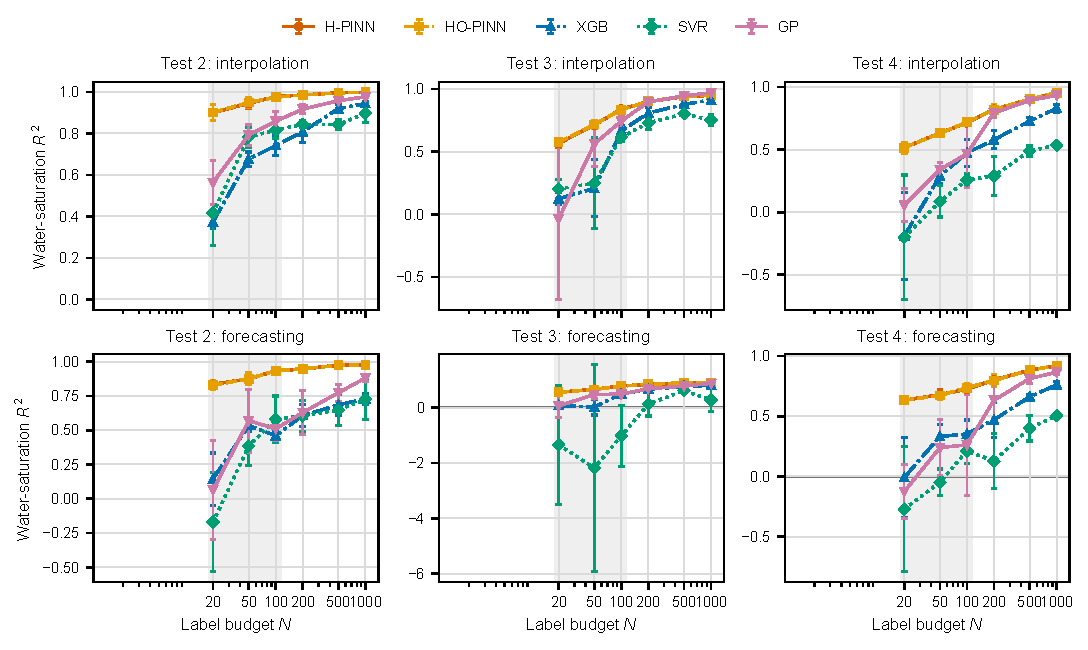
\includegraphics[width=\textwidth]{jcp_swat_r2_scaling.pdf}
    \caption{Water-saturation \(R^2\) versus labelled-state budget. Points and error bars are the mean and sample standard deviation over seeds 101--103. The grey band marks the prespecified small-data range \(N\le100\). Labels occupy the first 70\% of time; forecasting is evaluated on the final 30\%. Classical flow models are tuned by forward-time validation at every budget.}
    \label{fig:swat_scaling}
\end{figure*}

The flow learning curves in Fig.~\ref{fig:swat_scaling} show both the advantage and its boundary. Test 2 is PINN-dominated at every budget, although the interpolation margin decreases from 0.337 at \(N=20\) to 0.022 at \(N=1000\). Test 3 has the clearest crossover: the best PINN leads GP by 0.372, 0.154, and 0.095 at \(N=20,50,100\), is nearly tied at \(N=200\), and is slightly behind at \(N=500\) and \(N=1000\). Test 4 remains PINN-dominated because the same labels must cover space, time, and four physical parameters; its interpolation margin decreases from 0.459 at \(N=20\) to 0.021 at \(N=1000\).

\begin{table}[t]
\centering
\scriptsize
\setlength{\tabcolsep}{2.3pt}
\caption{Discrete label equivalence at $N=50$. $N^*_{\rm class}$ is the smallest tested budget at which any classical mean reaches the best PINN mean. Ratios are relative to 50 PINN labels.}
\label{tab:label_equivalence}
\begin{tabular}{@{}llclc@{}}
\toprule
Test & Region & PINN $R^2$ & $N^*_{\rm class}$ & Ratio \\
\midrule
T1 & Interp. & 0.999 & 100 (GP) & 2$\times$ \\
T1 & Forecast & 0.972 & $>1000$ & $>20\times$ \\
T2 & Interp. & 0.949 & 500 (GP) & 10$\times$ \\
T2 & Forecast & 0.876 & 1000 (GP) & 20$\times$ \\
T3 & Interp. & 0.716 & 100 (GP) & 2$\times$ \\
T3 & Forecast & 0.657 & 200 (GP) & 4$\times$ \\
T4 & Interp. & 0.633 & 200 (GP) & 4$\times$ \\
T4 & Forecast & 0.680 & 500 (GP) & 10$\times$ \\
\bottomrule
\end{tabular}
\end{table}


Table~\ref{tab:label_equivalence} expresses the same effect in label units. To match the best \(N=50\) PINN mean, a classical model requires 2--20 times more labels over seven of the eight test--region pairs. None reaches the heat-forecasting target by \(N=1000\). This is a discrete diagnostic over the tested budgets, not an interpolated sample-complexity estimate.

\begin{figure*}[t]
    \centering
    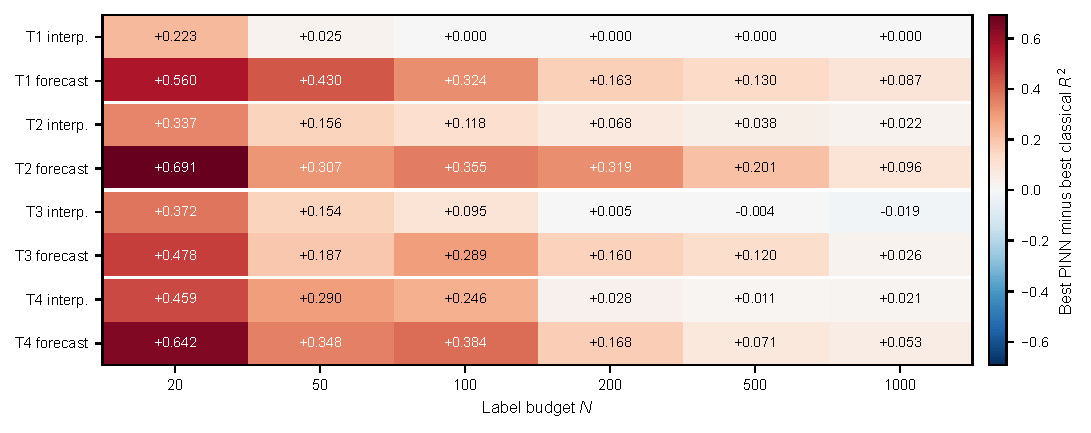
\includegraphics[width=\textwidth]{jcp_advantage_map.pdf}
    \caption{Difference between the best PINN and best classical mean \(R^2\) at every tested budget. Test 1 uses temperature; Tests 2--4 use water saturation. Positive values favour PINN.}
    \label{fig:advantage}
\end{figure*}

The advantage map in Fig.~\ref{fig:advantage} summarizes all 48 budget--test--region comparisons. The best PINN wins 43. All five classical wins are confined to interpolation: three negligible differences in the nearly solved heat problem and two Test 3 GP crossovers. A PINN has the highest mean in every temporal-forecasting comparison.

\begin{figure*}[t]
    \centering
    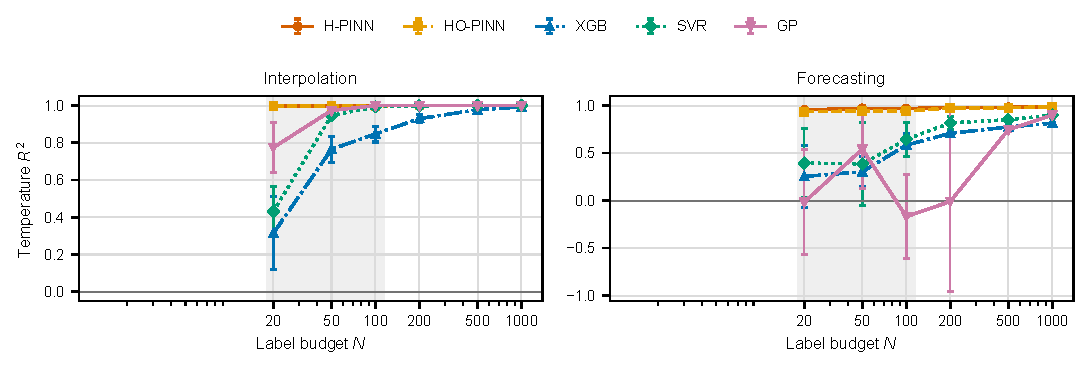
\includegraphics[width=\textwidth]{jcp_test1_r2_scaling.pdf}
    \caption{Temperature \(R^2\) for the analytical heat equation. The grey band marks \(N\le100\). GP becomes essentially exact for data-rich interpolation, whereas the PINN retains a clear equation-assisted forecasting advantage.}
    \label{fig:heat_scaling}
\end{figure*}

Figure~\ref{fig:heat_scaling} separates interpolation from forecasting on the smoothest benchmark. GP becomes essentially exact for interpolation from \(N=200\), but its future-time predictions remain unstable across sparse selections. H-PINN stays between 0.955 and 0.983 through \(N=20\)--500 because it enforces the heat operator beyond the latest labelled time.

\subsection{Qualitative reconstruction and physical admissibility}

\begin{figure}[H]
    \centering
    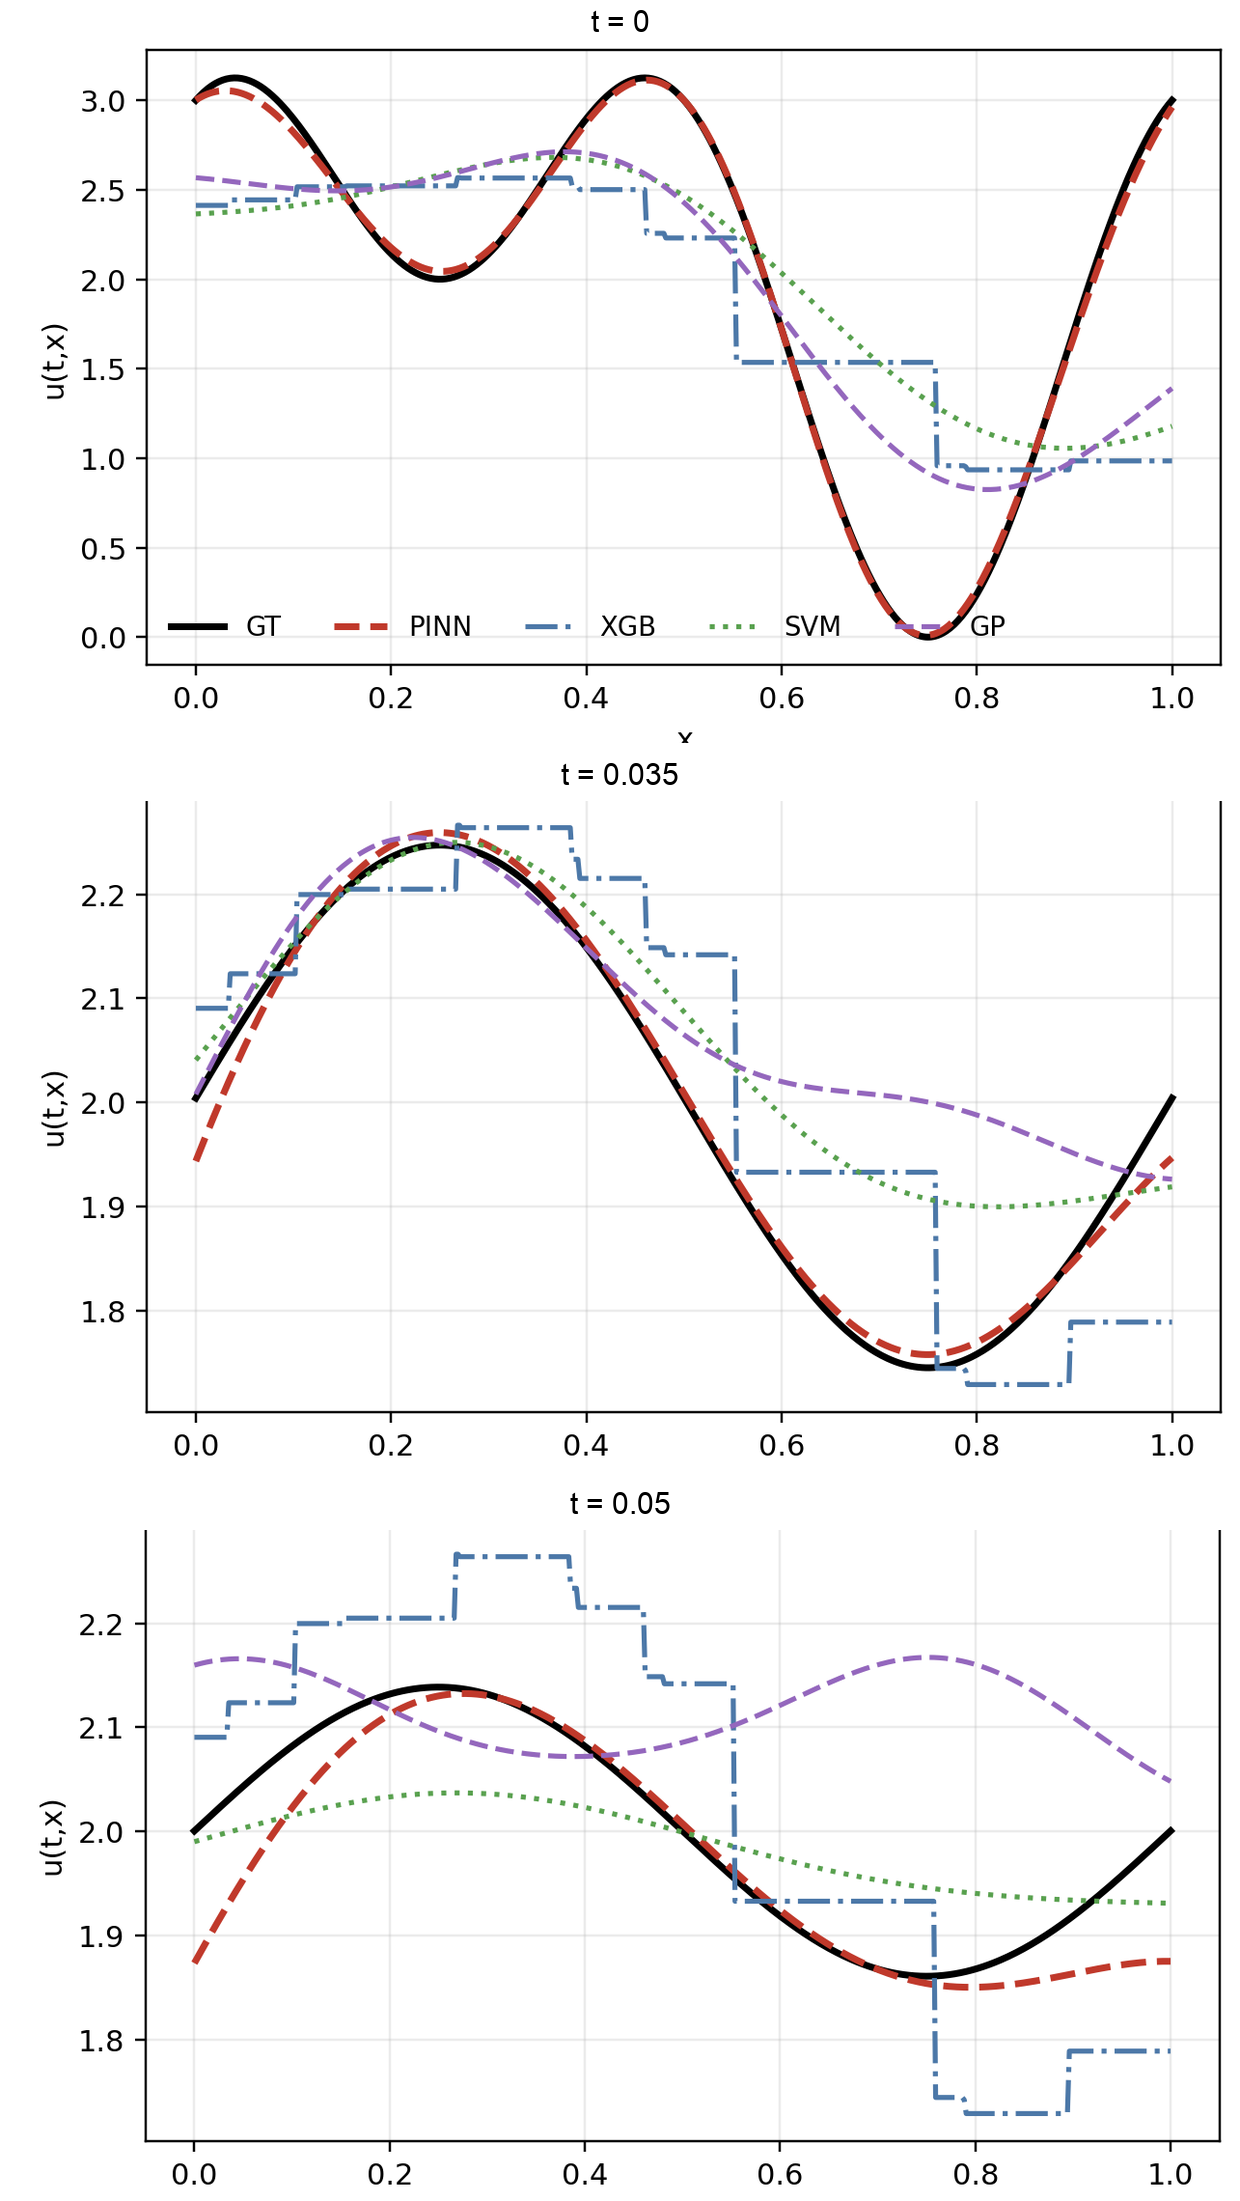
\includegraphics[width=0.90\columnwidth]{qualitative_test1_vertical.png}
    \caption{Test 1 profiles for seed 101 at \(N=20\): initial state (\(t=0\)), end of the labelled-time interval (\(t=0.035\)), and final forecast (\(t=0.05\)). H-PINN reconstructs the periodic modes and their dissipative evolution; XGB, SVR, and GP use the same labels but no equation residual.}
    \label{fig:qual_heat}
\end{figure}

The profiles in Fig.~\ref{fig:qual_heat} explain the heat scores. H-PINN preserves the correct modal decay from only 20 labels. XGB retains a piecewise-constant structure, while SVR and GP interpolate the observed interval smoothly but do not reproduce the final-time decay.

\begin{strip}
    \centering
    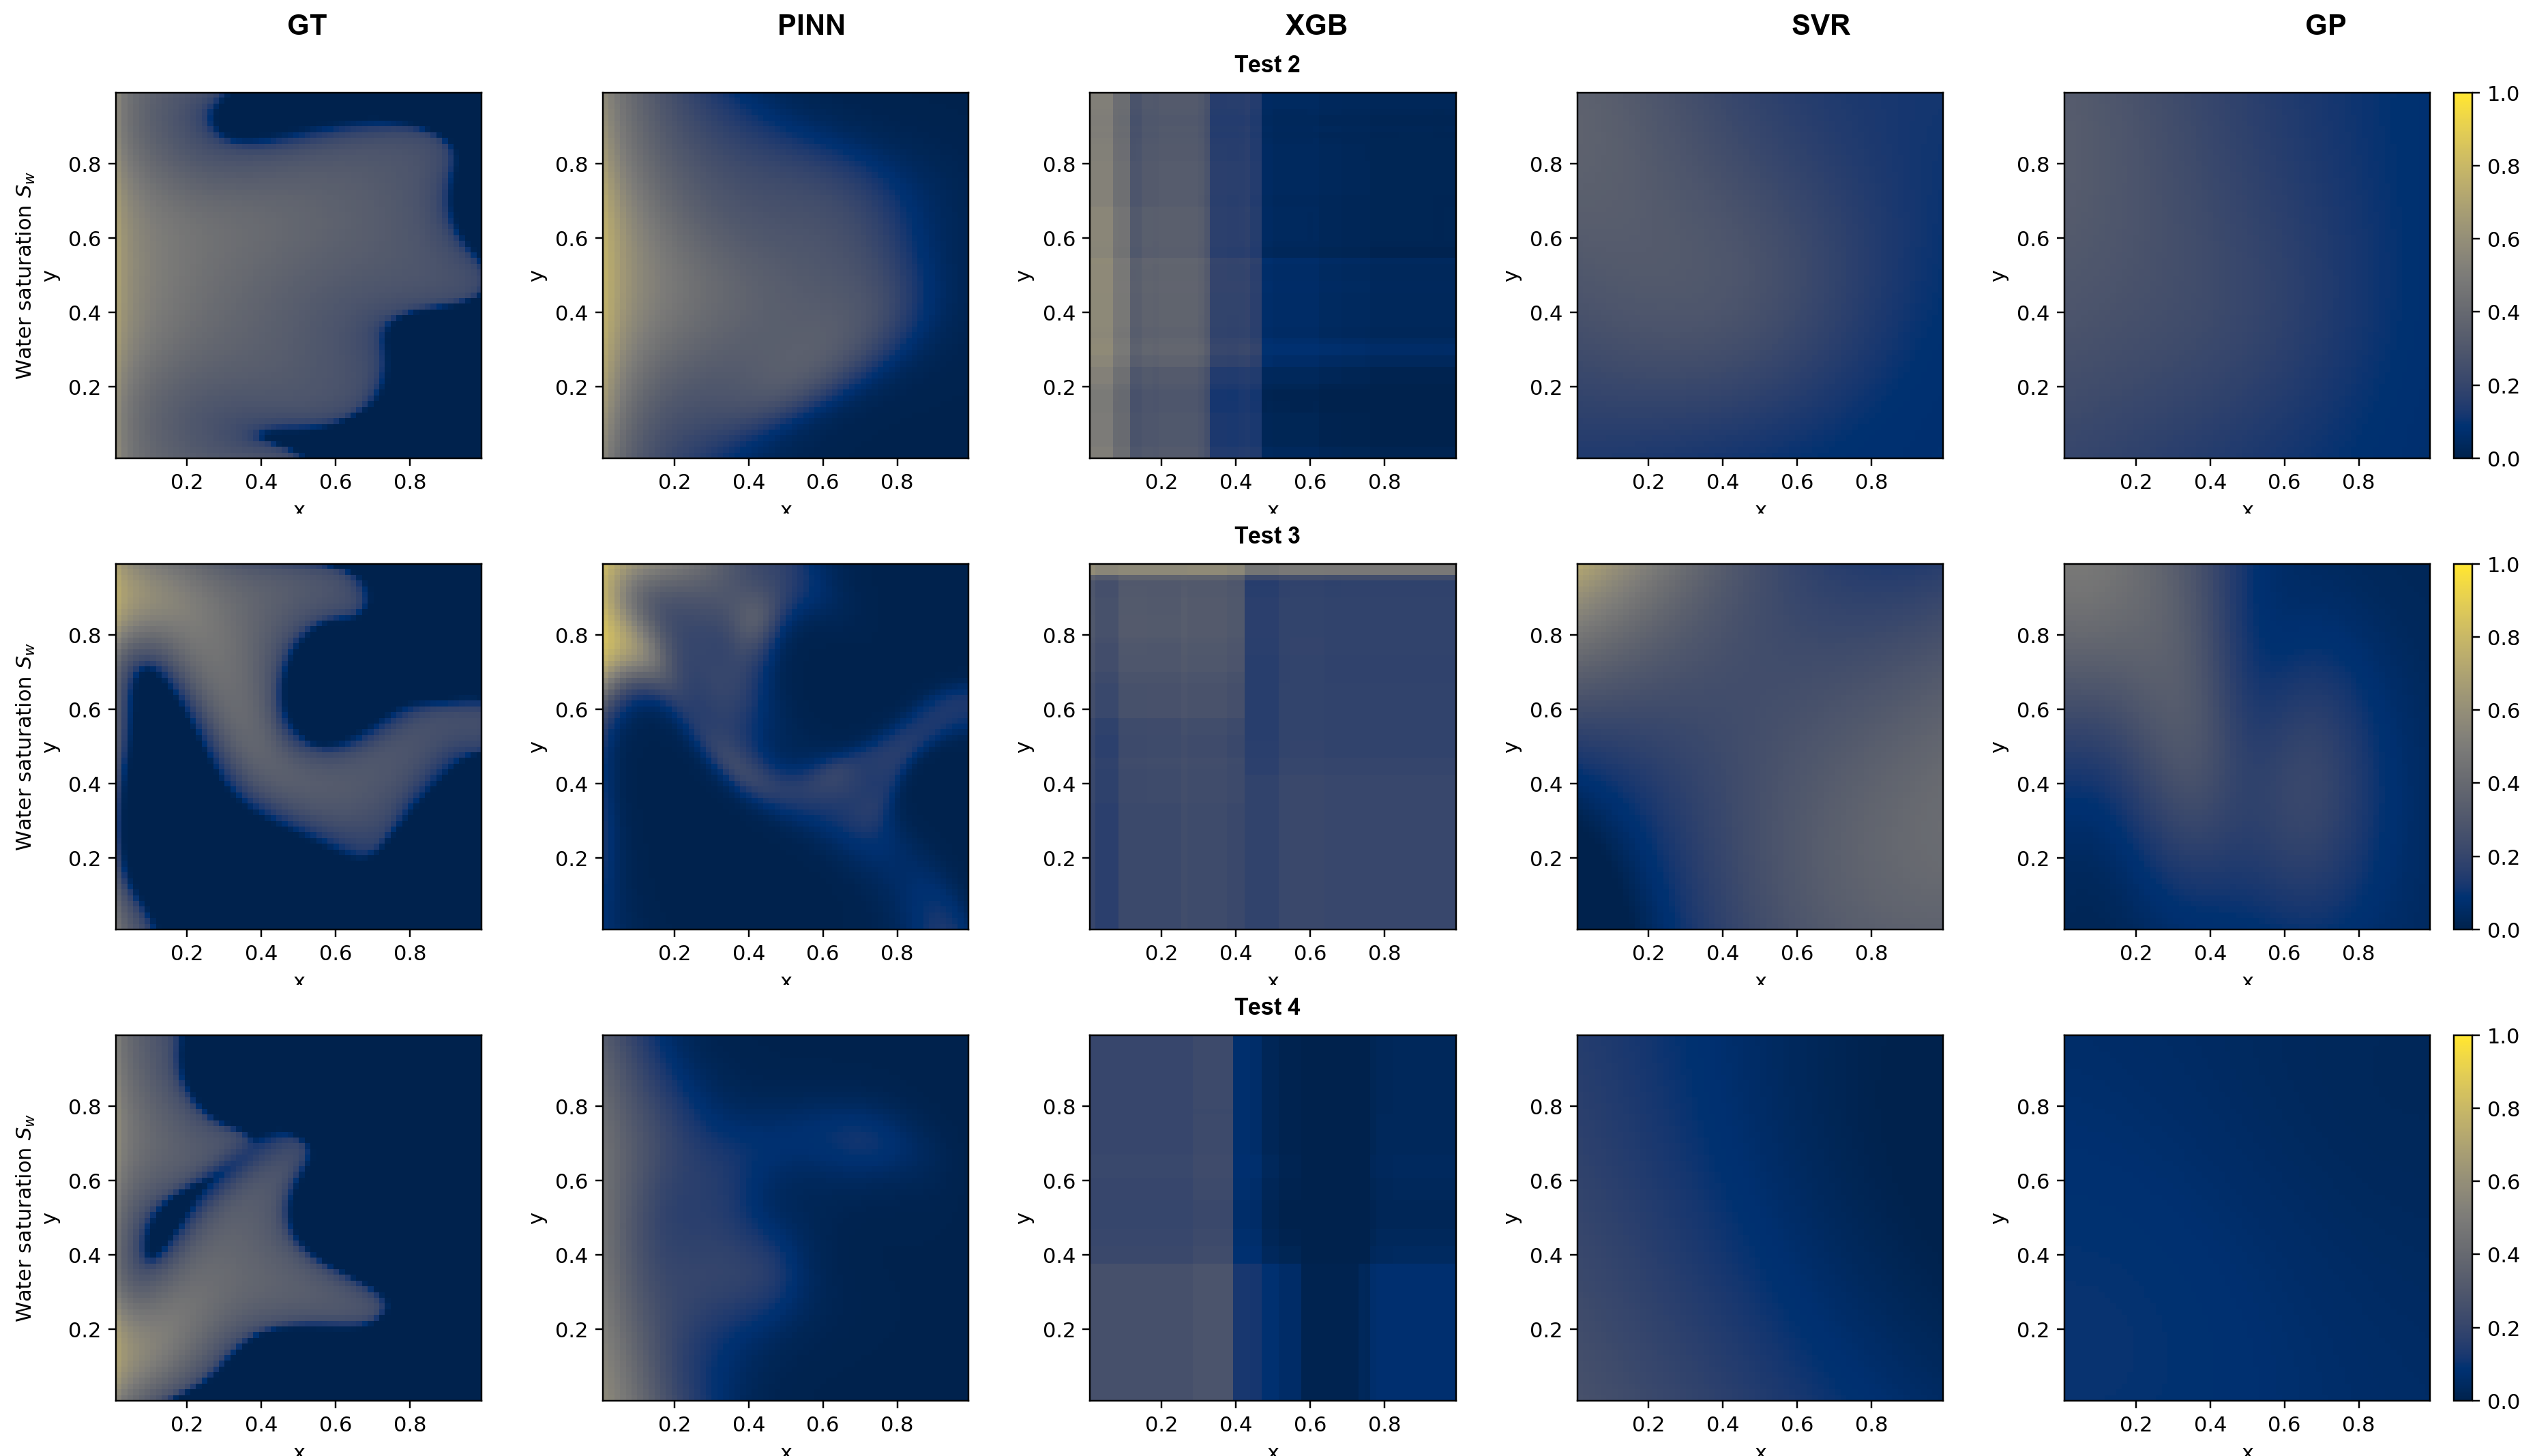
\includegraphics[width=0.96\textwidth]{qualitative_flow_saturation_composite.png}
    \captionsetup{hypcap=false}
    \captionof{figure}{Final forecasting-time water saturation for seed 101. Rows show Tests 2--4; columns compare the reference, H-PINN, XGB, SVR, and GP. Tests 2 and 3 use \(N=50\); Test 4 uses \(N=20\) and parameter realization 7. Colour limits are shared within every row.}
    \label{fig:qual_flow_saturation}
\end{strip}

The saturation fields in Fig.~\ref{fig:qual_flow_saturation} expose differences hidden by the easier pressure target (Appendix Fig.~\ref{fig:qual_flow_pressure}). H-PINN captures the displaced volume and broad front geometry in Test 2. In Test 3 it recovers the curved high-conductivity pathway; XGB is block-like, while SVR and GP smooth away much of the transported phase.

The Test 4 row is deliberately severe: 20 labelled states cannot explicitly cover 100 parameter combinations and a space--time domain. The classical saturation fields remain close to a low-amplitude average response. H-PINN does not reproduce every sharp feature, but predicts substantial displacement and its parameter-conditioned geometry, consistent with the positive forecasting \(R^2\).

The constrained output map gives zero saturation-bound violations in every flow run and closure MAE of approximately \(10^{-8}\). At \(N=50\), classical bounds-violation rates in the forecasting region range from 5.2\% to 18.6\% in Test 2, 3.7\% to 15.7\% in Test 3, and 1.3\% to 10.8\% in Test 4. These diagnostics (Table~\ref{tab:physical_diagnostics}) do not enter the accuracy ranking; they show that the PINN prediction is also physically admissible.

\subsection{Loss balancing and computational cost}

H-PINN and HO-PINN track one another closely throughout Fig.~\ref{fig:swat_scaling}. Neither uniformly dominates: HO-PINN is slightly better in several very sparse cases, whereas H-PINN is often equal or marginally stronger as \(N\) grows. The large scientific contrast is between either PINN and the classical models, not between the weighting variants. The simpler H-PINN alone has a higher mean than every classical baseline in all 24 comparisons at \(N\le100\).

The gain is not free. At \(N=50\), H-PINN fitting takes approximately 135--288 seconds and HO-PINN 216--448 seconds on the recorded hardware; complete classical tuning takes less than eight seconds and often less than one (Table~\ref{tab:runtime}). Thus, PINN is attractive when the cost of labels dominates
\begin{equation}
    C_{\mathrm{total}}(N)
    =N C_{\mathrm{label}}+C_{\mathrm{fit}}(N)+M C_{\mathrm{query}}(N),
\end{equation}
and the reduction in required \(N\) offsets the larger fitting cost. When labels are cheap and abundant, a tuned classical surrogate is operationally preferable.

\section{Discussion}
\label{sec:discussion}

\subsection{What the experiments establish}

The evidence supports a precise rather than universal statement:
\begin{quote}
\emph{For the tested PDEs, when the equation and boundary data are trusted and only 20--100 solution states are labelled, physics-informed training is substantially more accurate than tuned XGB, RBF-SVR, and GP, especially for transport-dominated water saturation and future-time prediction.}
\end{quote}
This statement is supported across four systems, two evaluation regions, six budgets, and three paired seeds. It is also robust to using H-PINN or HO-PINN. The strongest evidence is not a single favourable split but the repeated pattern: large positive margins at \(N=20\), smaller margins as \(N\) increases, and an interpretable GP crossover in data-richer interpolation.

The result should not be paraphrased as a claim that neural networks always outperform classical models. In Test 3 interpolation, GP is slightly better from \(N=500\). In the heat equation, GP becomes essentially exact once it has enough in-range observations. These cases are scientifically useful because they show when a conventional surrogate has acquired enough data for the physics prior to add little predictive value.

\subsection{Why the gain is largest in forecasting and saturation}

Sparse classical regression sees only input--output pairs. Beyond the latest labelled time it has no direct representation of conservation, diffusion, or Darcy transport. H/HO-PINN continues to constrain temporal derivatives and flux divergence throughout the domain, which explains why its advantage is larger in the final 30\% of time. This is also why the correct term is \emph{physics-assisted forecasting}: the future state is hidden, but the future operator is not.

Water saturation is the decisive target because it contains a moving, permeability-controlled front. Pressure is elliptic and spatially smooth, and therefore comparatively easy for GP and SVR. A macro-average would allow near-perfect pressure to mask a poor estimate of transported water. Reporting \(S_w\) separately makes the practical difficulty visible and aligns the metric with the most demanding component of the numerical solution.

\subsection{Fairness and limitations}

The comparison is intentionally favourable to the classical baselines in several respects. They use the same labels, their flow hyperparameters are chosen independently per target by forward-time cross-validation, and the search cost is included. No future evaluation value is used for tuning. Conversely, the PINN receives genuine extra prior information: the exact PDE, coefficients at residual points, and boundary conditions. This is not data leakage; it is the mechanism being evaluated. It does mean that the conclusion applies only when the governing model is available and sufficiently accurate.

Four limitations remain. First, there are only three final seeds, and the same numerical seeds were used during the staged PINN screen. The corrected flow fields were generated later and the configuration was frozen across them, but these are still post-selection reproducibility runs rather than an untouched confirmatory sample. Fine distinctions between H-PINN and HO-PINN or between nearly saturated models should not be interpreted as significance tests. Second, Tests 2--4 inherit the spatial and temporal error of one \(64^2\) finite-volume discretization. Grid refinement and comparison against laboratory data are natural next steps. Third, residual points cover the complete time interval. A strict extrapolation study in which both labels and residuals stop at \(0.7t_{\max}\) would answer a different question and is not claimed here. Fourth, the width/depth pair was fixed rather than systematically searched; \ref{app:tuning} distinguishes the completed activation and optimization screens from this architectural choice.

The study also does not compare alternative neural operators, PINN architectures, or numerical solvers. Those methods address broader methodological questions, whereas the present JCP study isolates a practical choice between one frozen physics-informed surrogate and established non-neural small-data regressors. Finally, permeability is assumed known as a PDE coefficient at queried coordinates. Uncertain fields, model-form error, noisy boundary conditions, and inverse identification require separate evaluation.

\section{Conclusions}
\label{sec:conclusion}

We evaluated whether PINNs offer a practical small-data advantage using identical labelled states, nested budgets, paired seeds, disjoint interpolation and forecasting tests, and strong training-only classical tuning. The answer is positive within a clearly defined regime. H-PINN has a higher mean primary \(\Rtwo\) than the strongest of XGB, RBF-SVR, and GP in every comparison at 20, 50, and 100 labels. For heterogeneous flow, the advantage is driven by the hardest quantity---water saturation---rather than by smooth pressure. A PINN also leads every temporal-forecasting comparison from 20 to 1000 labels and produces exactly admissible phase saturations.

As labels become more abundant, the margins shrink. GP slightly surpasses the PINN for Test 3 interpolation at 500--1000 labels, while the heat interpolation problem becomes essentially solved by both. This crossover is the expected boundary of the small-data hypothesis: equation residuals are most valuable when labelled coverage is insufficient.

PINNs require one to three orders of magnitude more fitting time than the tuned classical models in these experiments. Their benefit is therefore label efficiency, not optimizer efficiency. When solution labels require expensive simulation or measurement and the governing PDE is reliable, that trade-off can favour a PINN. When labels are plentiful or fitting latency dominates, a tuned classical surrogate remains the appropriate choice.


\FloatBarrier
\appendix
\section{Model selection and additional diagnostics}

\subsection{PINN architecture and optimization screening}
\label{app:tuning}

The final PINN configuration was obtained by a staged sensitivity study, not by optimizing on the final six-budget table. Each recorded development run used Tests 1--4, budgets \(N\in\{50,200\}\), seeds 101--103, and 5,000 epochs unless stated otherwise. At each stage we inspected interpolation and extrapolation primary \(R^2\), RMSE, physics-validation residuals, run-to-run variation, and cost. A candidate was retained before moving to the next stage. This procedure is substantially cheaper than the full Cartesian product, but it does not estimate interactions between all hyperparameters.

Table~\ref{tab:pinn_screen} lists the candidate sets reconstructed from the stored experiment namespaces and checkpoint metadata. The gated residual backbone with width 128 and six hidden layers was fixed before the recorded comparison. In particular, only this width/depth pair survives in the unified experiment archive; we therefore do not claim a systematic width/depth grid search. The activation comparison was complete for tanh, SiLU, and GELU, and GELU had the strongest pooled primary \(R^2\) across the development rows. The later stages retained \(L^0_{\mathrm{data}}=0.03\), \(L^0_{\mathrm{ibc}}=0.003\), HO floor \(c=0.25\), \(N_r/N=2\), and initial learning rate \(3\times10^{-3}\). Training was then extended from 5,000 to 10,000 epochs.

\begin{table*}[!htbp]
\centering
\small
\setlength{\tabcolsep}{3pt}
\caption{Recorded sequential PINN screening. Values in bold are used in the final experiments. The gate search was staged, so the listed values were not evaluated as one Cartesian product.}
\label{tab:pinn_screen}
\begin{tabular}{p{0.19\textwidth}p{0.52\textwidth}p{0.20\textwidth}}
\toprule
Stage & Values represented in completed experiment namespaces & Retained value\\
\midrule
Backbone size & Width 128, depth 6; no completed alternative width/depth grid in the unified archive & \textbf{128 / 6}\\
Activation & tanh, SiLU, GELU, with H-PINN and HO-PINN & \textbf{GELU}\\
Data gate target & \(L^0_{\mathrm{data}}\in\{0.01,0.03,0.1,0.3\}\) across staged runs & \textbf{0.03}\\
IBC gate target & \(L^0_{\mathrm{ibc}}\in\{0.001,0.003,0.01,0.03\}\) across staged runs & \textbf{0.003}\\
HO orthogonal floor & \(c\in\{0,0.25,0.5,0.75,1\}\); \(c=1\) is H-PINN weighting & \textbf{0.25}\\
Residual density & \(N_r/N\in\{1,2,4\}\), freshly resampled each epoch & \textbf{2}\\
Initial learning rate & \(\{3\times10^{-4},3\times10^{-3},10^{-2}\}\), cosine decay to \(10^{-5}\) & \textbf{\(3\times10^{-3}\)}\\
Epoch budget & 5,000 in screening; 10,000 in the reported runs & \textbf{10,000}\\
Optimizer and checkpoint & Adam; gradient clipping at 1; minimum detached balanced training loss & \textbf{fixed}\\
\bottomrule
\end{tabular}
\end{table*}

The stored activation runs give pooled development primary \(R^2\) values of 0.575, 0.596, and 0.618 for tanh, SiLU, and GELU, respectively, when averaging both PINN variants, all four tests, both regions, both development budgets, and three seeds. These pooled numbers are diagnostic only: they mix tasks with different response ranges and were never reported as a scientific performance metric. For the HO floor, the corresponding pooled values are 0.657, 0.658, 0.654, 0.657, and 0.655 for \(c=0,0.25,0.5,0.75,1\), showing that the choice of 0.25 is a shallow optimum rather than a decisive effect.

Selection of the gate targets was based on joint inspection rather than a preregistered scalar objective. For example, \(L^0_{\mathrm{ibc}}=0.001\) gives a slightly higher pooled development primary \(R^2\) than 0.003, while 0.003 was retained as the compromise used in the subsequent residual-density and learning-rate studies. We report this detail because choosing a retrospective scalar aggregation would overstate the precision of the tuning procedure. The final values should be interpreted as one robust common configuration, not a proof that each scalar is globally optimal.

The numerical seeds 101--103 were reused in the final table. The flow reference solutions were subsequently replaced by the corrected conservative generator, and the selected configuration was not retuned per corrected flow test, per budget, or per region. This reduces direct adaptation to Tests 2--4 but does not create an independent confirmatory seed set. Future work should repeat the frozen configuration on additional seeds and independently generated permeability fields.

\subsection{Classical-baseline hyperparameter searches}

Every classical candidate is fitted only on the current labelled set. Tests 2--4 use three strictly forward expanding-window folds; each validation block is later than its training block. Searches are performed independently for pressure, oil saturation, and water saturation, with negative MSE as the selection score. Input scaling and, for strong-profile SVR, target scaling are fitted within each fold.

\begin{table*}[!htbp]
\centering
\small
\setlength{\tabcolsep}{3pt}
\caption{Classical search spaces. The strong profile is used for Tests 2--4 at every budget and seed. Test 1 uses the standard profile described in the last row.}
\label{tab:classical_search}
\begin{tabular}{p{0.12\textwidth}p{0.69\textwidth}p{0.12\textwidth}}
\toprule
Method & Strong-profile candidates & Evaluated\\
\midrule
XGB & \(n_{\rm est}\in\{100,300,600,1000\}\), depth \(\in\{2,3,4,6\}\), learning rate \(\in\{0.01,0.03,0.05,0.1\}\), child weight \(\in\{1,3,5\}\), subsample \(\in\{0.7,0.85,1\}\), feature fraction \(\in\{0.7,0.9,1\}\), \(\ell_1\in\{0,0.01,0.1\}\), \(\ell_2\in\{0.1,1,10\}\) & 32 random\\
RBF-SVR & \(C\in\{0.1,1,10,100,1000\}\), \(\gamma\in\{\text{scale},\text{auto},0.01,0.03,0.1,0.3,1,3,10\}\), \(\epsilon\in\{10^{-4},10^{-3},10^{-2},0.03,0.05,0.1\}\) & 40 random\\
GP & Constant-scaled RBF, Mat\'ern-3/2, Mat\'ern-5/2, or rational-quadratic kernel, each with white noise; nugget \(\alpha\in\{10^{-8},10^{-6},10^{-4}\}\) & 12 grid\\
Test 1 & XGB: \(2\times2\times2=8\) estimator/depth/rate combinations; SVR: \(3\times3=9\) \(C/\gamma\) combinations with \(\epsilon=10^{-3}\); anisotropic RBF GP optimized by marginal likelihood & standard\\
\bottomrule
\end{tabular}
\end{table*}

The selected parameter dictionary, fold count, candidate count, and cross-validation score are serialized in each classical result row. Consequently, ``training-only tuned'' means that hyperparameters were selected inside the labelled training subset; it does not mean that defaults were used. Neither interpolation nor extrapolation evaluation values enter these searches.

\subsection{Complete primary comparison}
\label{app:primary_tables}

Tables~\ref{tab:primary_full_n20} and \ref{tab:primary_full_n100} report all five methods at the two budgets summarized in Table~\ref{tab:primary_summary}. They are separated by budget to preserve a normal reading orientation and a legible numerical font.

\begin{table*}[t]
\centering
\scriptsize
\setlength{\tabcolsep}{3.2pt}
\caption{Complete primary $R^2$ comparison at $N=20$ (mean $\pm$ sample standard deviation over seeds 101--103). Test 1 uses temperature; Tests 2--4 use water saturation. Bold marks the highest mean in each row.}
\label{tab:primary_full_n20}
\begin{tabular}{@{}llccccc@{}}
\toprule
Test & Region & H-PINN & HO-PINN & XGB & SVR & GP \\
\midrule
T1 & Interp. & \textbf{$0.997\pm0.002$} & $0.997\pm0.002$ & $0.314\pm0.195$ & $0.431\pm0.132$ & $0.775\pm0.132$ \\
T1 & Forecast & \textbf{$0.955\pm0.016$} & $0.936\pm0.030$ & $0.254\pm0.323$ & $0.395\pm0.363$ & $-0.015\pm0.552$ \\
\addlinespace[1pt]
T2 & Interp. & $0.900\pm0.038$ & \textbf{$0.901\pm0.038$} & $0.375\pm0.033$ & $0.417\pm0.158$ & $0.564\pm0.105$ \\
T2 & Forecast & \textbf{$0.834\pm0.027$} & $0.828\pm0.034$ & $0.143\pm0.191$ & $-0.171\pm0.361$ & $0.063\pm0.362$ \\
\addlinespace[1pt]
T3 & Interp. & $0.567\pm0.031$ & \textbf{$0.576\pm0.027$} & $0.125\pm0.049$ & $0.204\pm0.076$ & $-0.038\pm0.641$ \\
T3 & Forecast & $0.547\pm0.051$ & \textbf{$0.547\pm0.041$} & $0.070\pm0.088$ & $-1.344\pm2.152$ & $0.056\pm0.416$ \\
\addlinespace[1pt]
T4 & Interp. & \textbf{$0.517\pm0.044$} & $0.516\pm0.044$ & $-0.189\pm0.346$ & $-0.199\pm0.497$ & $0.058\pm0.129$ \\
T4 & Forecast & $0.632\pm0.017$ & \textbf{$0.632\pm0.019$} & $-0.009\pm0.330$ & $-0.271\pm0.520$ & $-0.126\pm0.226$ \\
\bottomrule
\end{tabular}
\end{table*}

\begin{table*}[t]
\centering
\scriptsize
\setlength{\tabcolsep}{3.2pt}
\caption{Complete primary $R^2$ comparison at $N=100$ (mean $\pm$ sample standard deviation over seeds 101--103). Test 1 uses temperature; Tests 2--4 use water saturation. Bold marks the highest mean in each row.}
\label{tab:primary_full_n100}
\begin{tabular}{@{}llccccc@{}}
\toprule
Test & Region & H-PINN & HO-PINN & XGB & SVR & GP \\
\midrule
T1 & Interp. & \textbf{$1.000\pm0.000$} & $0.999\pm0.001$ & $0.847\pm0.043$ & $0.993\pm0.004$ & \textbf{$1.000\pm0.000$} \\
T1 & Forecast & \textbf{$0.969\pm0.009$} & $0.943\pm0.038$ & $0.584\pm0.121$ & $0.645\pm0.180$ & $-0.168\pm0.441$ \\
\addlinespace[1pt]
T2 & Interp. & \textbf{$0.977\pm0.009$} & $0.975\pm0.009$ & $0.741\pm0.047$ & $0.816\pm0.040$ & $0.859\pm0.045$ \\
T2 & Forecast & $0.933\pm0.011$ & \textbf{$0.933\pm0.014$} & $0.460\pm0.030$ & $0.579\pm0.171$ & $0.511\pm0.084$ \\
\addlinespace[1pt]
T3 & Interp. & \textbf{$0.840\pm0.014$} & $0.836\pm0.022$ & $0.666\pm0.041$ & $0.616\pm0.035$ & $0.745\pm0.052$ \\
T3 & Forecast & \textbf{$0.780\pm0.052$} & $0.771\pm0.055$ & $0.491\pm0.072$ & $-1.021\pm1.095$ & $0.483\pm0.126$ \\
\addlinespace[1pt]
T4 & Interp. & $0.715\pm0.008$ & \textbf{$0.720\pm0.017$} & $0.474\pm0.108$ & $0.258\pm0.052$ & $0.466\pm0.266$ \\
T4 & Forecast & $0.725\pm0.037$ & \textbf{$0.737\pm0.038$} & $0.353\pm0.116$ & $0.212\pm0.102$ & $0.262\pm0.419$ \\
\bottomrule
\end{tabular}
\end{table*}


\subsection{Additional error and physical metrics}
\label{app:additional_metrics}

The main text reports target-resolved MSE and \(R^2\). Table~\ref{tab:test1_secondary} and Tables~\ref{tab:secondary_test2}--\ref{tab:secondary_test4} add RMSE, MAE, relative \(L^2\), and standard-deviation-normalized RMSE at \(N=50\). The definitions are
\begin{align}
\mathrm{RMSE}&=\sqrt{\mathrm{MSE}},
&\mathrm{MAE}&=\frac1m\sum_i|y_i-\widehat y_i|,\\
\mathrm{relative}\ L^2&=\frac{\lVert\boldsymbol y-\widehat{\boldsymbol y}\rVert_2}{\lVert\boldsymbol y\rVert_2},
&\mathrm{NRMSE}_{\mathrm{std}}&=\frac{\mathrm{RMSE}}{\operatorname{std}(\boldsymbol y)}.
\end{align}
The oil-saturation results and every seed-level value remain in the machine-readable \texttt{final\_results\_used.csv}; duplicating all six budgets and all three flow targets in print would obscure rather than clarify the primary comparison.

\begin{table*}[!htbp]
\centering
\small
\setlength{\tabcolsep}{3.2pt}
\caption{Complete Test 1 metrics at $N=50$ (mean $\pm$ sample standard deviation over seeds 101--103).}
\label{tab:test1_secondary}
\textbf{(a) Absolute errors}\par\smallskip
\begin{tabular}{llccc}
\toprule
Region & Method & MSE & RMSE & MAE \\
\midrule
Interp. & H-PINN & $\num{2.12e-04}\,\pm\,\num{1.62e-04}$ & 0.0139\,$\pm$\,0.0053 & 0.0093\,$\pm$\,0.0035 \\
Interp. & HO-PINN & $\num{2.27e-04}\,\pm\,\num{2.02e-04}$ & 0.0141\,$\pm$\,0.0063 & 0.0091\,$\pm$\,0.0039 \\
Interp. & XGB & $\num{5.10e-02}\,\pm\,\num{1.53e-02}$ & 0.2242\,$\pm$\,0.0335 & 0.1273\,$\pm$\,0.0142 \\
Interp. & SVM & $\num{1.16e-02}\,\pm\,\num{2.92e-03}$ & 0.1072\,$\pm$\,0.0138 & 0.0400\,$\pm$\,0.0061 \\
Interp. & GP & $\num{5.71e-03}\,\pm\,\num{5.72e-03}$ & 0.0696\,$\pm$\,0.0360 & 0.0252\,$\pm$\,0.0098 \\
\midrule
Extrap. & H-PINN & $\num{5.14e-04}\,\pm\,\num{2.58e-04}$ & 0.0221\,$\pm$\,0.0064 & 0.0139\,$\pm$\,0.0040 \\
Extrap. & HO-PINN & $\num{1.02e-03}\,\pm\,\num{6.87e-04}$ & 0.0308\,$\pm$\,0.0105 & 0.0190\,$\pm$\,0.0064 \\
Extrap. & XGB & $\num{1.26e-02}\,\pm\,\num{2.89e-03}$ & 0.1119\,$\pm$\,0.0132 & 0.0943\,$\pm$\,0.0128 \\
Extrap. & SVM & $\num{1.11e-02}\,\pm\,\num{7.97e-03}$ & 0.1014\,$\pm$\,0.0359 & 0.0827\,$\pm$\,0.0294 \\
Extrap. & GP & $\num{8.33e-03}\,\pm\,\num{7.55e-03}$ & 0.0856\,$\pm$\,0.0390 & 0.0651\,$\pm$\,0.0302 \\
\bottomrule
\end{tabular}
\par\medskip
\textbf{(b) Coefficient of determination and normalized errors}\par\smallskip
\begin{tabular}{llccc}
\toprule
Region & Method & $R^2$ & relative $L^2$ & NRMSE$_{\mathrm{std}}$ \\
\midrule
Interp. & H-PINN & 0.9990\,$\pm$\,0.0007 & 0.0068\,$\pm$\,0.0026 & 0.0299\,$\pm$\,0.0113 \\
Interp. & HO-PINN & 0.9990\,$\pm$\,0.0009 & 0.0069\,$\pm$\,0.0031 & 0.0304\,$\pm$\,0.0136 \\
Interp. & XGB & 0.7649\,$\pm$\,0.0706 & 0.1091\,$\pm$\,0.0163 & 0.4813\,$\pm$\,0.0719 \\
Interp. & SVM & 0.9464\,$\pm$\,0.0135 & 0.0522\,$\pm$\,0.0067 & 0.2302\,$\pm$\,0.0295 \\
Interp. & GP & 0.9737\,$\pm$\,0.0264 & 0.0339\,$\pm$\,0.0175 & 0.1495\,$\pm$\,0.0772 \\
\midrule
Extrap. & H-PINN & 0.9717\,$\pm$\,0.0142 & 0.0110\,$\pm$\,0.0032 & 0.1636\,$\pm$\,0.0473 \\
Extrap. & HO-PINN & 0.9439\,$\pm$\,0.0378 & 0.0153\,$\pm$\,0.0052 & 0.2282\,$\pm$\,0.0777 \\
Extrap. & XGB & 0.3049\,$\pm$\,0.1590 & 0.0558\,$\pm$\,0.0066 & 0.8299\,$\pm$\,0.0979 \\
Extrap. & SVM & 0.3874\,$\pm$\,0.4383 & 0.0506\,$\pm$\,0.0179 & 0.7519\,$\pm$\,0.2664 \\
Extrap. & GP & 0.5417\,$\pm$\,0.4154 & 0.0427\,$\pm$\,0.0195 & 0.6345\,$\pm$\,0.2893 \\
\bottomrule
\end{tabular}
\end{table*}

\begin{table*}[t]
\centering
\scriptsize
\setlength{\tabcolsep}{2.7pt}
\caption{Secondary error metrics for Test 2 at $N=50$ (mean $\pm$ sample standard deviation over seeds 101--103).}
\label{tab:secondary_test2}
\begin{tabular}{@{}cllcccc@{}}
\toprule
Target & Region & Method & RMSE & MAE & Relative $L^2$ & NRMSE$_{\rm std}$ \\
\midrule
$p$ & Interp. & H & $0.0062\pm0.0019$ & $0.0034\pm0.0007$ & $0.0101\pm0.0031$ & $0.0178\pm0.0055$ \\
$p$ & Interp. & HO & $0.0059\pm0.0016$ & $0.0033\pm0.0005$ & $0.0097\pm0.0026$ & $0.0170\pm0.0045$ \\
$p$ & Interp. & XGB & $0.0582\pm0.0100$ & $0.0431\pm0.0069$ & $0.0947\pm0.0163$ & $0.1666\pm0.0287$ \\
$p$ & Interp. & SVR & $0.0696\pm0.0029$ & $0.0577\pm0.0024$ & $0.1132\pm0.0047$ & $0.1993\pm0.0082$ \\
$p$ & Interp. & GP & $0.0172\pm0.0032$ & $0.0117\pm0.0013$ & $0.0280\pm0.0053$ & $0.0493\pm0.0093$ \\
\addlinespace[1pt]
$p$ & Forecast & H & $0.0124\pm0.0019$ & $0.0088\pm0.0012$ & $0.0193\pm0.0030$ & $0.0347\pm0.0053$ \\
$p$ & Forecast & HO & $0.0118\pm0.0012$ & $0.0085\pm0.0009$ & $0.0183\pm0.0018$ & $0.0328\pm0.0033$ \\
$p$ & Forecast & XGB & $0.0566\pm0.0053$ & $0.0419\pm0.0033$ & $0.0880\pm0.0082$ & $0.1580\pm0.0147$ \\
$p$ & Forecast & SVR & $0.1050\pm0.0303$ & $0.0860\pm0.0271$ & $0.1632\pm0.0472$ & $0.2930\pm0.0847$ \\
$p$ & Forecast & GP & $0.0245\pm0.0054$ & $0.0183\pm0.0034$ & $0.0381\pm0.0085$ & $0.0685\pm0.0152$ \\
\addlinespace[1pt]
\midrule
$S_w$ & Interp. & H & $0.0360\pm0.0089$ & $0.0151\pm0.0043$ & $0.2014\pm0.0499$ & $0.2305\pm0.0571$ \\
$S_w$ & Interp. & HO & $0.0347\pm0.0075$ & $0.0144\pm0.0035$ & $0.1944\pm0.0422$ & $0.2225\pm0.0483$ \\
$S_w$ & Interp. & XGB & $0.0887\pm0.0047$ & $0.0620\pm0.0056$ & $0.4968\pm0.0266$ & $0.5684\pm0.0304$ \\
$S_w$ & Interp. & SVR & $0.0725\pm0.0081$ & $0.0500\pm0.0037$ & $0.4060\pm0.0456$ & $0.4646\pm0.0522$ \\
$S_w$ & Interp. & GP & $0.0706\pm0.0091$ & $0.0469\pm0.0047$ & $0.3958\pm0.0511$ & $0.4528\pm0.0585$ \\
\addlinespace[1pt]
$S_w$ & Forecast & H & $0.0652\pm0.0108$ & $0.0420\pm0.0082$ & $0.2275\pm0.0376$ & $0.3510\pm0.0580$ \\
$S_w$ & Forecast & HO & $0.0649\pm0.0109$ & $0.0408\pm0.0076$ & $0.2265\pm0.0379$ & $0.3494\pm0.0584$ \\
$S_w$ & Forecast & XGB & $0.1267\pm0.0060$ & $0.1010\pm0.0080$ & $0.4418\pm0.0209$ & $0.6817\pm0.0322$ \\
$S_w$ & Forecast & SVR & $0.1451\pm0.0170$ & $0.1171\pm0.0172$ & $0.5061\pm0.0594$ & $0.7809\pm0.0917$ \\
$S_w$ & Forecast & GP & $0.1193\pm0.0316$ & $0.0919\pm0.0264$ & $0.4160\pm0.1101$ & $0.6418\pm0.1699$ \\
\addlinespace[1pt]
\bottomrule
\end{tabular}
\end{table*}

\begin{table*}[t]
\centering
\scriptsize
\setlength{\tabcolsep}{2.7pt}
\caption{Secondary error metrics for Test 3 at $N=50$ (mean $\pm$ sample standard deviation over seeds 101--103).}
\label{tab:secondary_test3}
\begin{tabular}{@{}cllcccc@{}}
\toprule
Target & Region & Method & RMSE & MAE & Relative $L^2$ & NRMSE$_{\rm std}$ \\
\midrule
$p$ & Interp. & H & $0.0283\pm0.0032$ & $0.0211\pm0.0019$ & $0.0532\pm0.0060$ & $0.0946\pm0.0107$ \\
$p$ & Interp. & HO & $0.0282\pm0.0042$ & $0.0209\pm0.0024$ & $0.0530\pm0.0078$ & $0.0944\pm0.0139$ \\
$p$ & Interp. & XGB & $0.0973\pm0.0067$ & $0.0728\pm0.0009$ & $0.1830\pm0.0126$ & $0.3258\pm0.0225$ \\
$p$ & Interp. & SVR & $0.1154\pm0.0068$ & $0.0899\pm0.0040$ & $0.2170\pm0.0128$ & $0.3863\pm0.0228$ \\
$p$ & Interp. & GP & $0.0539\pm0.0174$ & $0.0355\pm0.0107$ & $0.1014\pm0.0327$ & $0.1806\pm0.0582$ \\
\addlinespace[1pt]
$p$ & Forecast & H & $0.0449\pm0.0058$ & $0.0339\pm0.0044$ & $0.0781\pm0.0102$ & $0.1451\pm0.0189$ \\
$p$ & Forecast & HO & $0.0445\pm0.0049$ & $0.0338\pm0.0035$ & $0.0775\pm0.0084$ & $0.1440\pm0.0157$ \\
$p$ & Forecast & XGB & $0.0949\pm0.0072$ & $0.0737\pm0.0008$ & $0.1653\pm0.0125$ & $0.3073\pm0.0232$ \\
$p$ & Forecast & SVR & $0.1528\pm0.0331$ & $0.1251\pm0.0336$ & $0.2659\pm0.0576$ & $0.4943\pm0.1070$ \\
$p$ & Forecast & GP & $0.0639\pm0.0126$ & $0.0460\pm0.0079$ & $0.1112\pm0.0220$ & $0.2067\pm0.0408$ \\
\addlinespace[1pt]
\midrule
$S_w$ & Interp. & H & $0.0655\pm0.0028$ & $0.0316\pm0.0017$ & $0.4990\pm0.0214$ & $0.5350\pm0.0229$ \\
$S_w$ & Interp. & HO & $0.0651\pm0.0038$ & $0.0314\pm0.0022$ & $0.4961\pm0.0293$ & $0.5319\pm0.0314$ \\
$S_w$ & Interp. & XGB & $0.1082\pm0.0162$ & $0.0579\pm0.0030$ & $0.8243\pm0.1234$ & $0.8838\pm0.1323$ \\
$S_w$ & Interp. & SVR & $0.1036\pm0.0284$ & $0.0641\pm0.0189$ & $0.7891\pm0.2168$ & $0.8460\pm0.2324$ \\
$S_w$ & Interp. & GP & $0.0797\pm0.0179$ & $0.0422\pm0.0044$ & $0.6072\pm0.1361$ & $0.6510\pm0.1459$ \\
\addlinespace[1pt]
$S_w$ & Forecast & H & $0.0993\pm0.0049$ & $0.0617\pm0.0025$ & $0.4799\pm0.0237$ & $0.5853\pm0.0289$ \\
$S_w$ & Forecast & HO & $0.0996\pm0.0065$ & $0.0621\pm0.0041$ & $0.4816\pm0.0317$ & $0.5874\pm0.0386$ \\
$S_w$ & Forecast & XGB & $0.1669\pm0.0253$ & $0.1400\pm0.0275$ & $0.8069\pm0.1222$ & $0.9841\pm0.1491$ \\
$S_w$ & Forecast & SVR & $0.2690\pm0.1703$ & $0.2208\pm0.1448$ & $1.3001\pm0.8232$ & $1.5857\pm1.0040$ \\
$S_w$ & Forecast & GP & $0.1227\pm0.0177$ & $0.0940\pm0.0129$ & $0.5930\pm0.0856$ & $0.7233\pm0.1044$ \\
\addlinespace[1pt]
\bottomrule
\end{tabular}
\end{table*}

\begin{table*}[t]
\centering
\scriptsize
\setlength{\tabcolsep}{2.7pt}
\caption{Secondary error metrics for Test 4 at $N=50$ (mean $\pm$ sample standard deviation over seeds 101--103).}
\label{tab:secondary_test4}
\begin{tabular}{@{}cllcccc@{}}
\toprule
Target & Region & Method & RMSE & MAE & Relative $L^2$ & NRMSE$_{\rm std}$ \\
\midrule
$p$ & Interp. & H & $0.0161\pm0.0037$ & $0.0104\pm0.0025$ & $0.0258\pm0.0059$ & $0.0434\pm0.0100$ \\
$p$ & Interp. & HO & $0.0164\pm0.0034$ & $0.0105\pm0.0023$ & $0.0264\pm0.0055$ & $0.0444\pm0.0092$ \\
$p$ & Interp. & XGB & $0.1072\pm0.0108$ & $0.0780\pm0.0044$ & $0.1723\pm0.0173$ & $0.2893\pm0.0291$ \\
$p$ & Interp. & SVR & $0.1401\pm0.0241$ & $0.1045\pm0.0186$ & $0.2251\pm0.0388$ & $0.3779\pm0.0652$ \\
$p$ & Interp. & GP & $0.0316\pm0.0048$ & $0.0209\pm0.0028$ & $0.0507\pm0.0078$ & $0.0852\pm0.0130$ \\
\addlinespace[1pt]
$p$ & Forecast & H & $0.0231\pm0.0040$ & $0.0148\pm0.0027$ & $0.0365\pm0.0064$ & $0.0611\pm0.0107$ \\
$p$ & Forecast & HO & $0.0223\pm0.0040$ & $0.0143\pm0.0025$ & $0.0353\pm0.0064$ & $0.0591\pm0.0107$ \\
$p$ & Forecast & XGB & $0.1061\pm0.0105$ & $0.0792\pm0.0028$ & $0.1679\pm0.0166$ & $0.2814\pm0.0278$ \\
$p$ & Forecast & SVR & $0.1740\pm0.0655$ & $0.1335\pm0.0523$ & $0.2753\pm0.1036$ & $0.4614\pm0.1736$ \\
$p$ & Forecast & GP & $0.0344\pm0.0056$ & $0.0239\pm0.0035$ & $0.0544\pm0.0089$ & $0.0911\pm0.0150$ \\
\addlinespace[1pt]
\midrule
$S_w$ & Interp. & H & $0.0661\pm0.0028$ & $0.0281\pm0.0018$ & $0.5666\pm0.0236$ & $0.6056\pm0.0253$ \\
$S_w$ & Interp. & HO & $0.0662\pm0.0025$ & $0.0280\pm0.0017$ & $0.5681\pm0.0215$ & $0.6073\pm0.0230$ \\
$S_w$ & Interp. & XGB & $0.0920\pm0.0038$ & $0.0519\pm0.0071$ & $0.7889\pm0.0325$ & $0.8433\pm0.0347$ \\
$S_w$ & Interp. & SVR & $0.1041\pm0.0073$ & $0.0694\pm0.0094$ & $0.8925\pm0.0625$ & $0.9541\pm0.0668$ \\
$S_w$ & Interp. & GP & $0.0884\pm0.0037$ & $0.0454\pm0.0084$ & $0.7582\pm0.0318$ & $0.8105\pm0.0340$ \\
\addlinespace[1pt]
$S_w$ & Forecast & H & $0.0919\pm0.0057$ & $0.0557\pm0.0044$ & $0.4687\pm0.0288$ & $0.5653\pm0.0347$ \\
$S_w$ & Forecast & HO & $0.0930\pm0.0047$ & $0.0561\pm0.0039$ & $0.4738\pm0.0242$ & $0.5715\pm0.0291$ \\
$S_w$ & Forecast & XGB & $0.1327\pm0.0102$ & $0.0928\pm0.0135$ & $0.6765\pm0.0520$ & $0.8160\pm0.0627$ \\
$S_w$ & Forecast & SVR & $0.1665\pm0.0090$ & $0.1211\pm0.0024$ & $0.8485\pm0.0458$ & $1.0234\pm0.0553$ \\
$S_w$ & Forecast & GP & $0.1408\pm0.0211$ & $0.0928\pm0.0129$ & $0.7177\pm0.1074$ & $0.8657\pm0.1296$ \\
\addlinespace[1pt]
\bottomrule
\end{tabular}
\end{table*}


\FloatBarrier
\clearpage

\begin{strip}
\centering
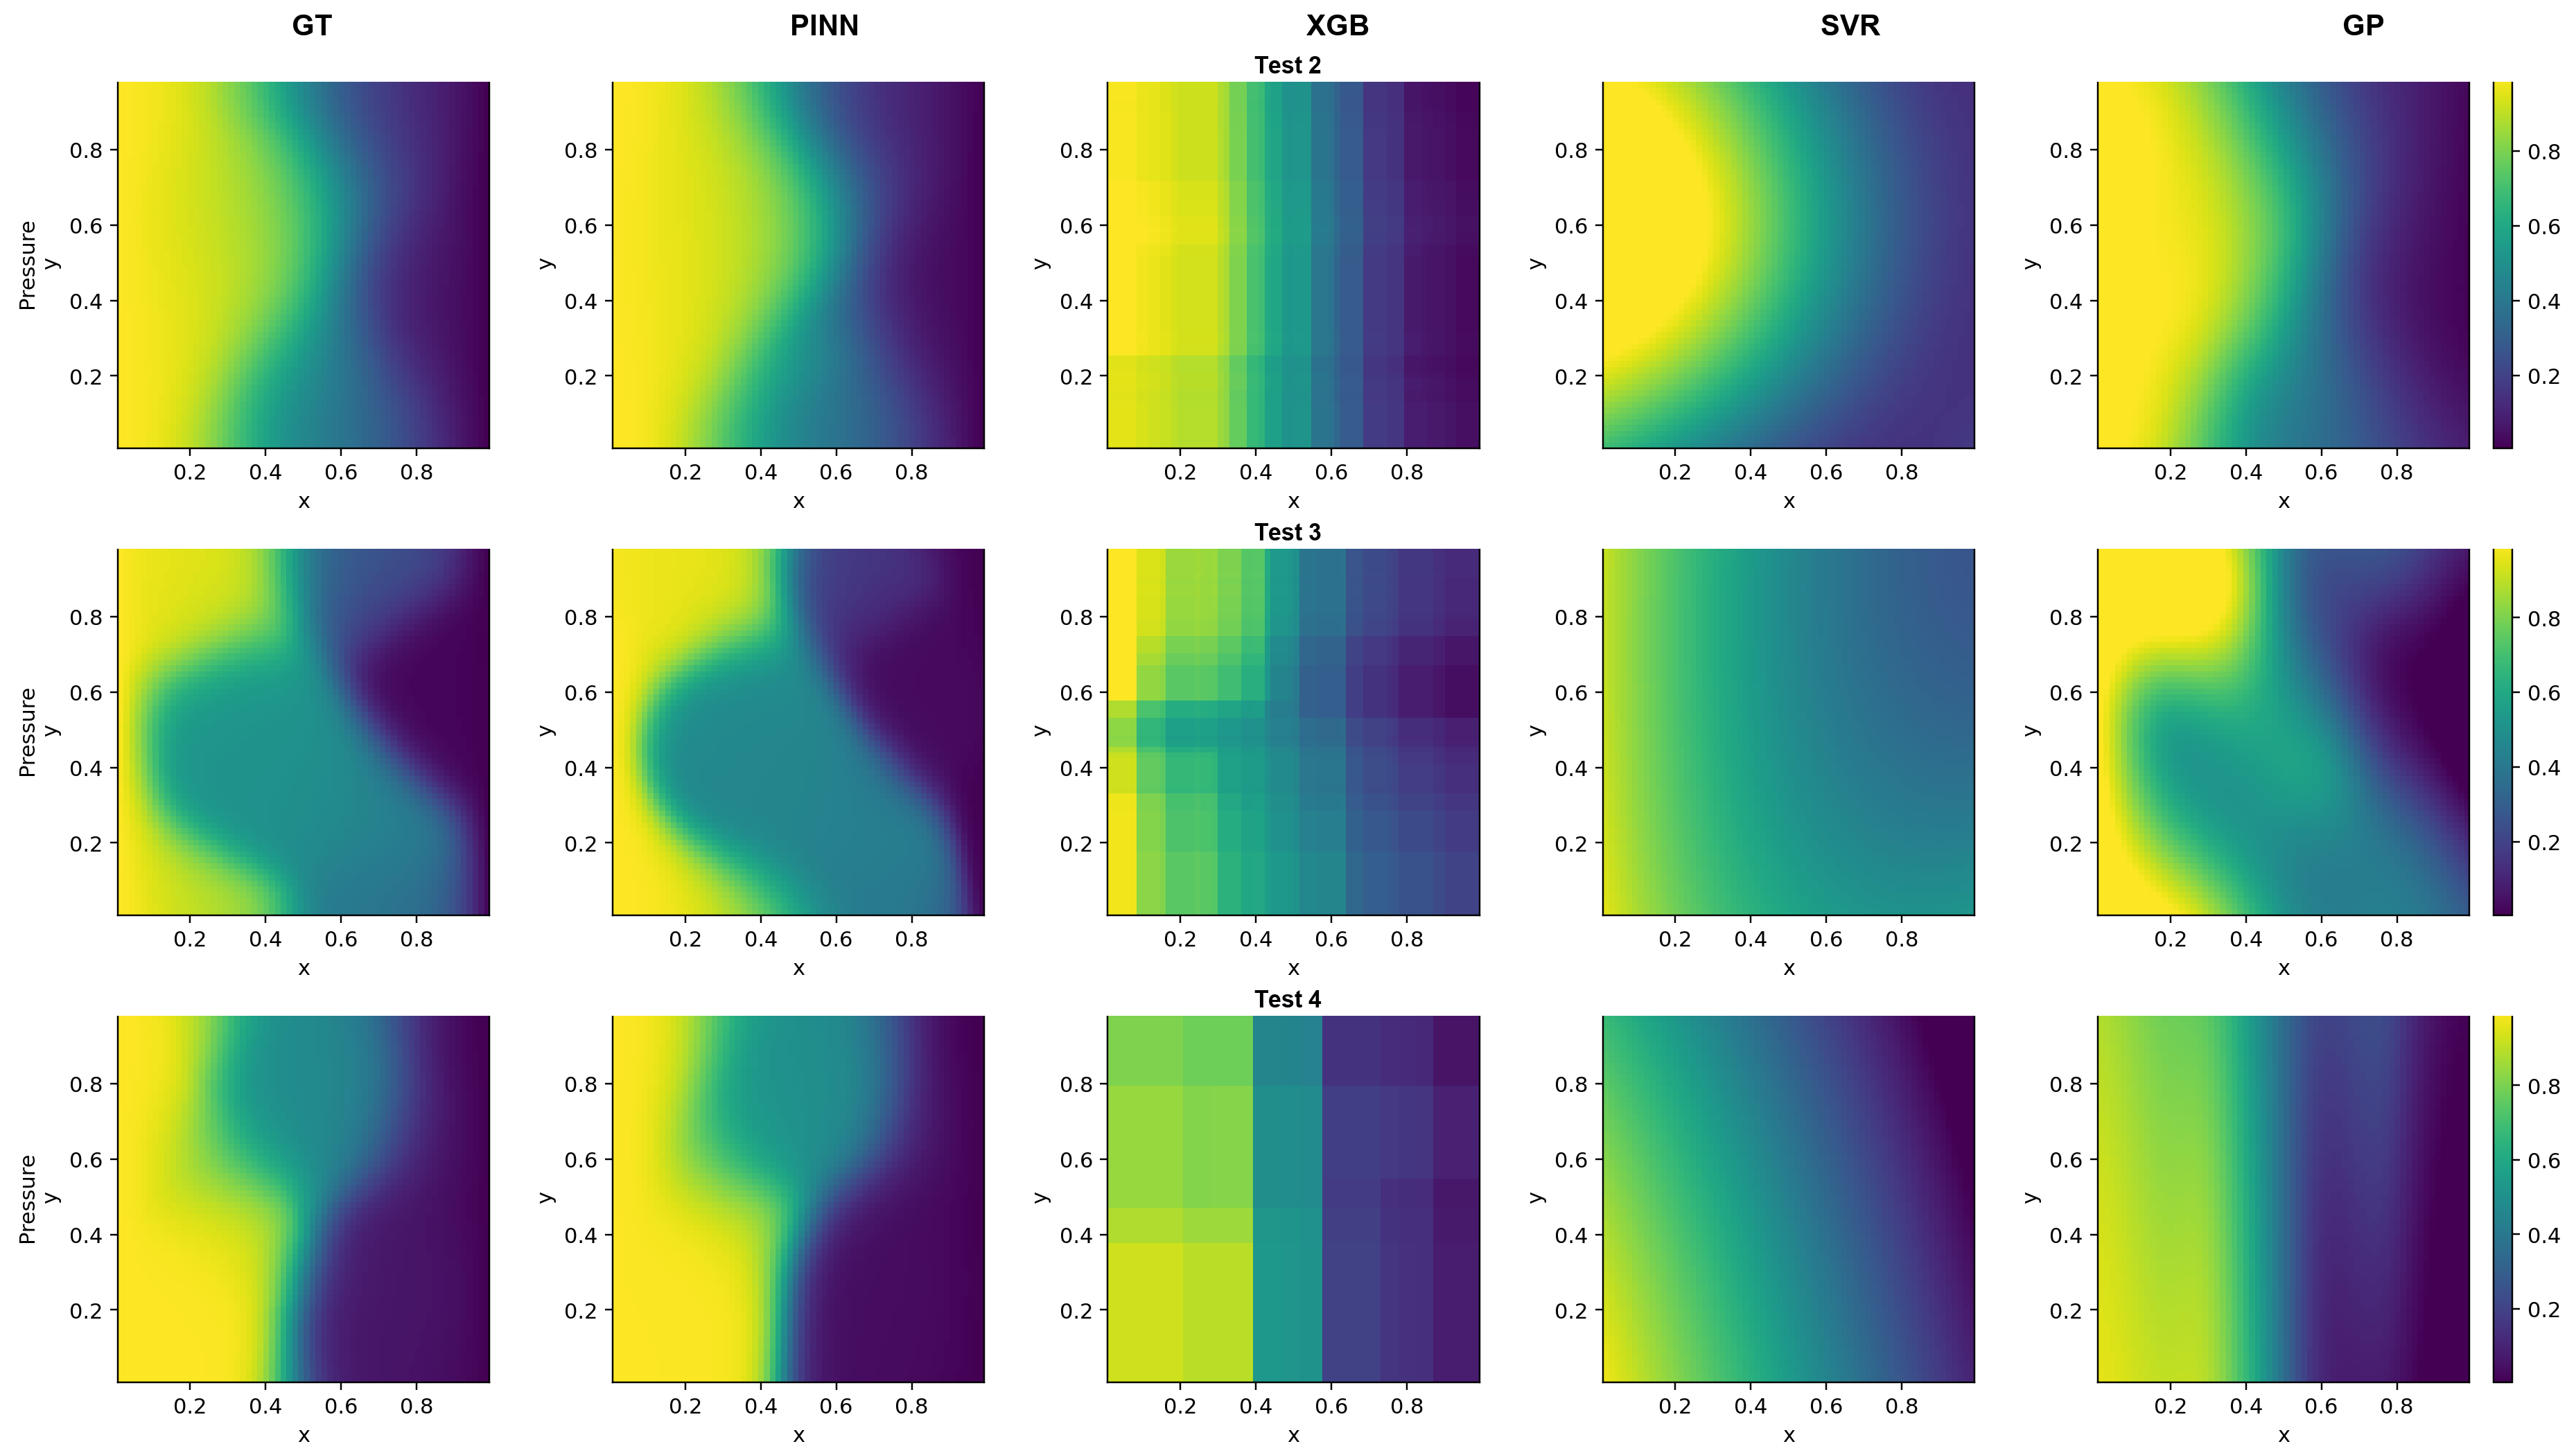
\includegraphics[width=0.94\textwidth]{qualitative_flow_pressure_composite.png}
\captionsetup{hypcap=false}
\captionof{figure}{Final forecasting-time pressure for seed 101. Rows show Tests 2--4; columns compare the reference, H-PINN, XGB, SVR, and GP. Tests 2 and 3 use \(N=50\); Test 4 uses \(N=20\) and parameter realization 7. Shared row-wise colour limits make the comparatively smooth pressure target directly comparable across methods.}
\label{fig:qual_flow_pressure}
\end{strip}

Pressure is smooth relative to transported saturation and is already close to saturated in the target-resolved scores of Table~\ref{tab:target_summary}. Figure~\ref{fig:qual_flow_pressure} confirms that all methods reproduce the dominant left-to-right trend, although XGB remains block-like and SVR suppresses heterogeneity. The visual comparison therefore supports reporting water saturation as the primary flow target rather than averaging it with the much easier pressure field.

\clearpage
\begin{table}[H]
\centering
\scriptsize
\setlength{\tabcolsep}{1.5pt}
\caption{Physical diagnostics in the forecasting region at $N=50$ (mean $\pm$ sample standard deviation). The violation rate is the fraction of predictions outside $[-10^{-3},1+10^{-3}]$ for either saturation; closure is $|\widehat S_w+\widehat S_o-1|$.}
\label{tab:physical_diagnostics}
\begin{tabular}{@{}llcc@{}}
\toprule
Test & Method & Violation rate & Closure MAE \\
\midrule
T2 & H & $0.0000\pm0.0000$ & $\num{9.59e-09}\pm\num{1.05e-09}$ \\
T2 & HO & $0.0000\pm0.0000$ & $\num{9.52e-09}\pm\num{3.61e-10}$ \\
T2 & XGB & $0.1231\pm0.0999$ & $\num{2.67e-02}\pm\num{7.93e-03}$ \\
T2 & SVR & $0.1858\pm0.1306$ & $\num{8.47e-03}\pm\num{6.24e-03}$ \\
T2 & GP & $0.0520\pm0.0747$ & $\num{2.14e-07}\pm\num{3.49e-07}$ \\
\addlinespace[1pt]
T3 & H & $0.0000\pm0.0000$ & $\num{1.02e-08}\pm\num{3.03e-09}$ \\
T3 & HO & $0.0000\pm0.0000$ & $\num{9.54e-09}\pm\num{2.42e-09}$ \\
T3 & XGB & $0.0527\pm0.0655$ & $\num{6.96e-02}\pm\num{3.09e-02}$ \\
T3 & SVR & $0.1573\pm0.0804$ & $\num{1.13e-02}\pm\num{9.49e-03}$ \\
T3 & GP & $0.0373\pm0.0419$ & $\num{1.75e-08}\pm\num{1.18e-08}$ \\
\addlinespace[1pt]
T4 & H & $0.0000\pm0.0000$ & $\num{8.09e-09}\pm\num{7.55e-10}$ \\
T4 & HO & $0.0000\pm0.0000$ & $\num{8.74e-09}\pm\num{1.11e-09}$ \\
T4 & XGB & $0.1078\pm0.1124$ & $\num{1.76e-02}\pm\num{2.83e-03}$ \\
T4 & SVR & $0.0133\pm0.0231$ & $\num{2.38e-03}\pm\num{2.06e-03}$ \\
T4 & GP & $0.0551\pm0.0512$ & $\num{1.32e-08}\pm\num{4.64e-09}$ \\
\bottomrule
\end{tabular}
\end{table}


\subsection{Computational cost}
Classical times include the complete target-wise hyperparameter search, while PINN times include automatic differentiation and checkpoint selection. Reference-solver generation is excluded for every surrogate because the same generated states define the common labelled pool.

\begin{table*}[!htbp]
\centering
\small
\setlength{\tabcolsep}{3.5pt}
\caption{Wall-clock fitting and tuning time in seconds at $N=50$ (mean $\pm$ sample standard deviation over three seeds). Classical times include hyperparameter selection; reference-data generation is excluded.}
\label{tab:runtime}
\begin{tabular}{lccccc}
\toprule
Test & H-PINN & HO-PINN & XGB & SVM & GP \\
\midrule
Test 1 & 134.52\,$\pm$\,18.86 & 216.36\,$\pm$\,31.72 & 0.30\,$\pm$\,0.00 & 0.08\,$\pm$\,0.00 & \textbf{0.07\,$\pm$\,0.02} \\
Test 2 & 279.91\,$\pm$\,68.78 & 417.58\,$\pm$\,42.82 & 4.48\,$\pm$\,0.45 & \textbf{0.61\,$\pm$\,0.03} & 3.20\,$\pm$\,0.16 \\
Test 3 & 229.22\,$\pm$\,21.09 & 447.80\,$\pm$\,160.06 & 4.05\,$\pm$\,0.38 & \textbf{0.62\,$\pm$\,0.01} & 5.63\,$\pm$\,0.27 \\
Test 4 & 287.82\,$\pm$\,79.38 & 421.88\,$\pm$\,73.71 & 4.57\,$\pm$\,0.43 & \textbf{0.56\,$\pm$\,0.01} & 7.74\,$\pm$\,2.40 \\
\bottomrule
\end{tabular}
\end{table*}



\section*{Data and code availability}
The repository contains the corrected finite-volume generator, unified training runner, stored experiment CSV files, checkpoints, labelled selections, and the script that regenerates every table and figure in this manuscript. A public archival URL and immutable release identifier will be inserted before submission.

\section*{CRediT authorship contribution statement}
\textbf{Kirill Katsuba:} Conceptualization, Methodology, Software, Investigation, Visualization, Writing -- original draft. \textbf{Oleg Rudenko:} Methodology, Validation, Writing -- review and editing. \textbf{Alexander Tarakanov:} Conceptualization, Supervision, Writing -- review and editing. Author roles will be confirmed before submission.

\section*{Declaration of competing interest}
The authors declare that they have no known competing financial interests or personal relationships that could have appeared to influence the work reported in this paper.

\section*{Funding}
Funding information will be added before submission.

\section*{Declaration of generative AI and AI-assisted technologies in the writing process}
During preparation of this work, the authors used OpenAI Codex for code-assisted analysis, LaTeX drafting, and language editing. The authors reviewed and edited all generated material and take full responsibility for the content of the publication.

\bibliographystyle{elsarticle-num}
\renewcommand{\bibfont}{\small}
\bibliography{references}

\end{document}
